% scritto da\AT{}
\section{Strategia di testing}
Il gruppo \Gruppo{}, per assicurarsi che il prodotto da realizzare sia corretto, intende effettuare un piano di testing delle componenti e del sistema software nel suo complesso.
L'obiettivo è seguire il \glo{modello a V} per correlare ogni attività di testing (parte destra della V) con la corrispondente attività della parte sinistra della V.

\begin{figure}[h]
    \centering
    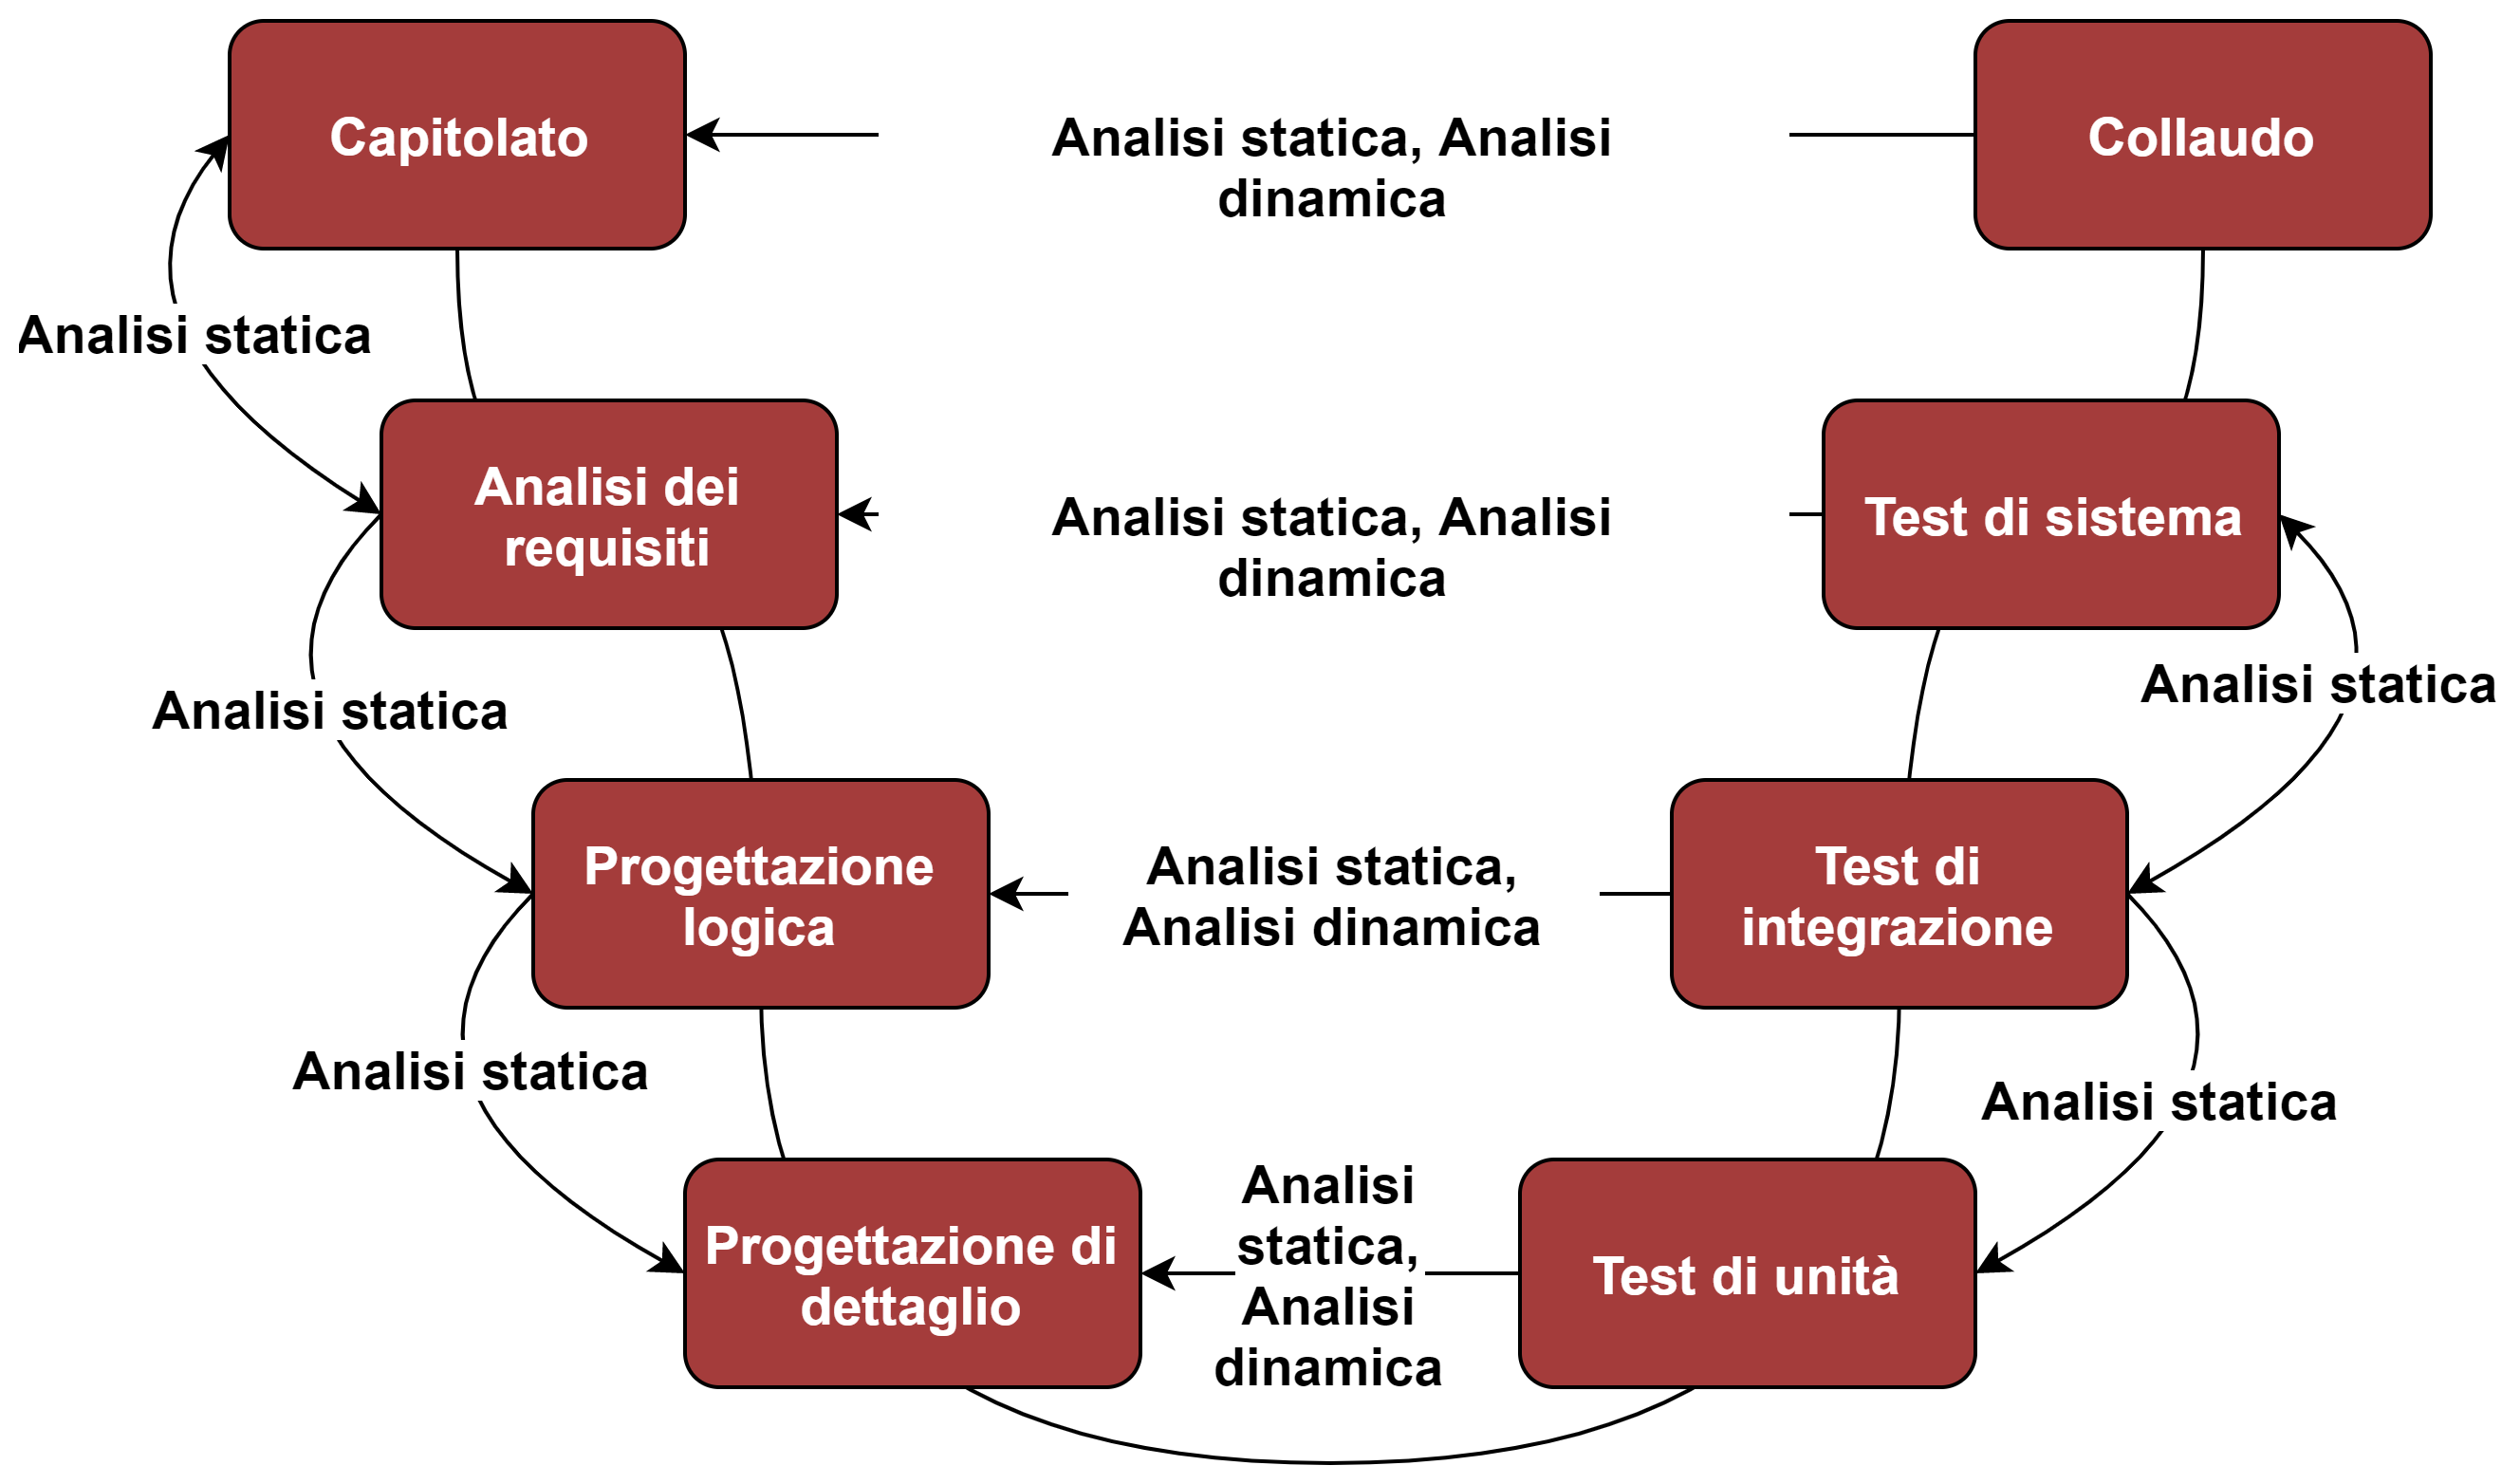
\includegraphics[scale=0.85]{Sezioni/Immagini/ModelloV.png}
    \caption{Modello a V}
\end{figure}

\subsection{Tipologie di test}
I test specificati dal \glo{modello a V} e che devono essere realizzati dal gruppo sono:
\begin{itemize}
    \item \textbf{Test di unità:} Verificano il corretto comportamento di una singola unità del programma. L'unità è una funzionalità atomica verificabile in modo isolato, in modo da assicurare che il risultato dei test su essa non siano influenzati dal comportamento di altre unità; 
    \item \textbf{Test di integrazione:} Verificano il corretto comportamento di più unità che devono cooperare per svolgere appieno i loro compiti;
    \item \textbf{Test di sistema:} Verificano il comportamento dell'intero sistema. I requisiti funzionali, di vincolo, di qualità e di prestazione concordati alla stipulazione del contratto con il committente devono essere soddisfatti per intero;
    \item \textbf{Test di accettazione:} Vengono eseguiti assieme al committente e il loro superamento permette di procedere con il rilascio del prodotto software.
\end{itemize}

\subsubsection{Test di unità}
Allo stato attuale del progetto non è possibile definire quali test di unità dovranno essere realizzati, in quanto devono essere realizzati in contemporanea alla progettazione di dettaglio.\\
Questa sezione del documento verrà redatta non appena inizierà l'attività di progettazione di dettaglio.

{
\rowcolors{2}{grigetto}{white}
\renewcommand{\arraystretch}{1.5}
\centering
\begin{longtable}{ c C{13cm} C{1cm}}
\caption{Elenco dei test di unità}\\
\rowcolor{darkblue}
\textcolor{white}{\textbf{Codice}} & \textcolor{white}{\textbf{Descrizione}} & \textcolor{white}{\textbf{Stato}}\\
\endfirsthead
\rowcolor{darkblue}
\textcolor{white}{\textbf{Codice}} & \textcolor{white}{\textbf{Descrizione}} & \textcolor{white}{\textbf{Stato}}\\
\endhead

TUA1 & Si verifichi che l'utente non \glo{autenticato} possa inserire l'indirizzo e-mail. & NI \\
TUA2 & Si verifichi che l'utente non \glo{autenticato} possa inserire la password. & NI \\
TUA3 & Si verifichi che l'utente non \glo{autenticato} possa ricevere un messaggio di errore se l'\glo{autenticazione} viene negata per inserimento di credenziali errate. & NI \\
TUA4 & Si verifichi che l'utente non \glo{autenticato} possa effettuare il reset della password qualora se la fosse dimenticata. & NI \\
TUA5 & Si verifichi che l’utente non \glo{autenticato} possa inserire l'indirizzo e-mail. & NI \\
TUA6 & Si verifichi che l’utente non \glo{autenticato} possa ricevere un messaggio di errore se tentasse di registrarsi con un'e-mail già usata nel sistema.  & NI \\
TUA7 & Si verifichi che l’utente non \glo{autenticato} possa inserire una password. & NI \\
TUA8 & Si verifichi che l’utente non \glo{autenticato} possa inserire nuovamente la password come conferma. & NI \\
TUA9 & Si verifichi che l’utente non \glo{autenticato} possa ricevere un messaggio di errore qualora abbia inserito una password non ritenuta sicura. Il processo di \glo{autenticazione} deve fallire. & NI \\
TUA10 & Si verifichi che l’utente non \glo{autenticato} possa ricevere un messaggio di errore qualora abbia inserito una conferma password diversa dalla password. Il processo di \glo{autenticazione} deve fallire. & NI \\
TUA11 & Si verifichi che l’utente non \glo{autenticato} possa accettare le condizioni generali d'uso. & NI \\
TUA12 & Si verifichi che la registrazione si interrompa e che l'applicazione si chiuda nel caso che l'utente non autenticato non abbia accettato le condizioni generali d'uso. & NI \\
TUA13 & Si verifichi che l'utente anonimo possa effettuare il \glo{logout} dall'applicazione. & NI \\
TUA14 & Si verifichi che l'utente anonimo possa scaricare la lista di tutte le organizzazioni. & NI \\
TUA15 & Si verifichi che l'utente anonimo riceva un messaggio di errore qualora lo scaricamento della lista di tutte le organizzazioni non vada a buon fine. & NI \\
TUA16 & Si verifichi che l'utente anonimo ossa aggiornare la lista delle organizzazioni tramite \glo{refresh manuale}. & NI \\
TUA17 & Si verifichi che l'utente anonimo possa aggiornare la lista delle organizzazioni tramite \glo{temporizzazione}. & NI \\
TUA18 & Si verifichi che l'utente anonimo possa visionare la lista delle organizzazioni ordinate alfabeticamente. & NI \\
TUA19 & Si verifichi che l'utente anonimo possa visionare la lista delle organizzazioni ordinate secondo la politica \glo{FIFO}. & NI \\
TUA20 & Si verifichi che l'utente anonimo possa visionare la lista delle organizzazioni che permettono il tracciamento anonimo. & NI \\
TUA21 & Si verifichi che l'utente anonimo possa visionare la lista delle organizzazioni che permettono il \glo{tracciamento autenticato}. & NI \\
TUA22 & Si verifichi che l'utente anonimo possa ricercare organizzazioni presenti nella lista delle organizzazioni appartenenti alle nazioni indicate dall'utente. & NI \\
TUA23 & Si verifichi che l'utente anonimo possa ricercare organizzazioni presenti nella lista delle organizzazioni che hanno nel nome una sottostringa scelta dall'utente. & NI \\
TUA24 & Si verifichi che l'utente anonimo possa ricercare organizzazioni presenti nella lista delle organizzazioni appartenenti alla città indicata dall'utente. & NI \\
TUA25 & Si verifichi che l'utente anonimo possa inserire un'organizzazione, presente nella lista di tutte le organizzazioni, nella propria lista delle organizzazioni preferite. & NI \\
TUA26 & Si verifichi che l'utente anonimo possa rimuovere un'organizzazione dalla propria lista delle organizzazioni preferite. & NI \\
TUA27 & Si verifichi che l'utente anonimo venga informato nel caso in cui non sia memorizzata nessuna lista delle organizzazioni del proprio dispositivo. & NI \\
TUA28 & Si verifichi che l'utente riconosciuto possa inserire la modalità di \glo{tracciamento anonimo}. & NI \\
TUA29 & Si verifichi che l'utente riconosciuto possa inserire la modalità di \glo{tracciamento autenticato}. & NI \\
TUA30 & Si verifichi che nel passaggio dalla modalità di \glo{tracciamento autenticato} a quella anonima venga inviata al sistema la richiesta di uscita dell'utente riconosciuto dal luogo e la successiva richiesta di ingresso di utente anonimo. & NI \\
TUA31 & Si verifichi che nel passaggio dalla modalità di \glo{tracciamento anonimo} a quella autenticata venga inviata al sistema la richiesta di uscita dell'utente anonimo dal luogo e la successiva richiesta di ingresso di utente riconosciuto. & NI \\
TUA32 & Si verifichi che l'utente anonimo possa vedere il proprio storico accessi presso un'\glo{organizzazione}. & NI \\
TUA33 & Si verifichi che ogni accesso deve mostrare la data in cui è stato compiuto. & NI \\
TUA34 & Si verifichi che ogni accesso deve mostrare il luogo corrispondente.  & NI \\
TUA35 & Si verifichi che ogni accesso deve mostrare il tempo totale trascorso all'interno nel luogo. & NI \\
TUA36 & Si verifichi che la \glo{lista degli accessi} deve risultare ordinata \glo{per data in ordine decrescente}. & NI \\
TUA37 & Si verifichi che la \glo{lista degli accessi} deve risultare ordinata \glo{per data in ordine crescente}. & NI \\
TUA38 & Si verifichi che nella lista vengono mostrati solo gli accessi che rispettano i parametri di ricerca sul giorno cercato. & NI \\
TUA39 & Si verifichi che l’utente anonimo riceva un messaggio informativo in assenza di accessi effettuati presso un'\glo{organizzazione}. & NI \\
TUA40 & Si verifichi che l’utente anonimo possa visionare il nome dello specifico luogo in cui si trova. & NI \\
TUA41 & Si verifichi che l’utente anonimo possa visionare il tempo trascorso da quando ha fatto l'ultimo ingresso in uno specifico luogo. & NI \\
TUA42 & Si verifichi che l'utente anonimo possa vedere il proprio storico accessi presso il luogo di un'\glo{organizzazione}. & NI \\
TUA43 & Si verifichi che ogni accesso deve mostrare la data in cui è stato compiuto. & NI \\
TUA44 & Si verifichi che ogni accesso deve mostrare il luogo corrispondente. & NI \\
TUA45 & Si verifichi che ogni accesso deve mostrare il tempo totale trascorso all'interno nel luogo. & NI \\
TUA46 & Si verifichi che la \glo{lista degli accessi} deve risultare ordinata \glo{per data in ordine decrescente}. & NI \\
TUA47 & Si verifichi che la \glo{lista degli accessi} deve risultare ordinata \glo{per data in ordine crescente}. & NI \\
TUA48 & Si verifichi che nella lista vengono mostrati solo gli accessi che rispettano i parametri di ricerca sul giorno cercato. & NI \\
TUA49 & Si verifichi che l'utente anonimo, in assenza di accessi effettuati presso il luogo di un'\glo{organizzazione} selezionato, visualizzi un messaggio informativo. & NI \\
TUA50 & Si verifichi che l'utente anonimo possa visualizzare il tempo trascorso all'interno del luogo dall'ultimo ingresso effettuato. & NI \\
TUA51 & Si verifichi che l’utente anonimo riceva la notifica della corretta registrazione se il tracciamento del suo \glo{movimento} in/da un \glo{luogo} ha avuto successo. & NI \\
TUA52 & Si verifichi che l’utente anonimo riceva un messaggio di errore qualora il tracciamento del \glo{movimento} non sia andato a buon fine. & NI \\
TUA53 & Si verifichi che durante la registrazione del \glo{tracciamento} del \glo{movimento} dell'utente anonimo/riconosciuto, venga memorizzato il \glo{timestamp} in cui è avvenuto il \glo{movimento}. & NI \\
TUA54 & Si verifichi che se l'utente riconosciuto è in modalità di \glo{tracciamento autenticato}, venga verificata la correttezza delle credenziali \glo{LDAP}. & NI \\
TUA55 & Si verifichi che se l'utente riconosciuto è in modalità di \glo{tracciamento autenticato}, possa effettuare un ingresso in un luogo dell'\glo{organizzazione}. & NI \\
TUA56 & Si verifichi che se l'utente riconosciuto è in modalità di \glo{tracciamento anonima}, possa effettuare un ingresso in un luogo dell'\glo{organizzazione}. & NI \\
TUA57 & Si verifichi che se l'utente riconosciuto è in modalità di \glo{tracciamento anonima}, possa effettuare un'uscita da un luogo dell'\glo{organizzazione}. & NI \\
TUA58 & Si verifichi che l’utente anonimo possa autenticarsi con credenziali aziendali LDAP in un'organizzazione che richiede il tracciamento riconosciuto. & NI \\
TUA59 & Si verifichi che l’utente anonimo riceva un messaggio di errore qualora le credenziali \glo{LDAP} non fossero riconosciute dal server. & NI \\
TUA60 & Si verifichi che l’utente anonimo possa inserire il proprio nome utente durante l'autenticazione con le credenziali \glo{LDAP} aziendali. & NI \\
TUA61 & Si verifichi che l’utente anonimo possa inserire la propria password utente durante l'autenticazione con le credenziali \glo{LDAP} aziendali. & NI \\
TUS1 & Si verifichi che l’utente non \glo{autenticato} possa inserire l'e-mail correttamente. & NI \\
TUS2 & Si verifichi che l’utente non \glo{autenticato} possa inserire correttamente la password. & NI \\
TUS3 & Si verifichi che l’utente non \glo{autenticato} riceva un messaggio d'errore se l'\glo{autenticazione} viene negata per inserimento di credenziali errate. & NI \\
TUS4 & Si verifichi che l’utente non \glo{autenticato} possa effettuare il reset della password qualora se la fosse dimenticata. & NI \\
TUS5 & Si verifichi che l'amministratore \glo{autenticato} possa effettuare il \glo{logout} dalla applicazione web. & NI \\
TUS6 & Si verifichi che l’amministratore visualizzatore possa selezionare un’organizzazione dalla sua lista delle organizzazioni. & NI \\
TUS7 & Si verifichi che l'amministratore visualizzatore possa visualizzare il nome dell'organizzazione selezionata. & NI \\
TUS8 & Si verifichi che l'amministratore visualizzatore possa visualizzare l’immagine dell'organizzazione selezionata. & NI \\
TUS9 & Si verifichi che l'amministratore visualizzatore possa visualizzare la descrizione dell'organizzazione selezionata. & NI \\
TUS10 & Si verifichi che l'amministratore visualizzatore possa visualizzare l’indirizzo dell'organizzazione selezionata. & NI \\
TUS11 & Si verifichi che l'amministratore visualizzatore possa visualizzare l’indirizzo IP dell'organizzazione selezionata. & NI \\
TUS12 & Si verifichi che l'amministratore visualizzatore possa visualizzare le coordinate geografiche dell'organizzazione selezionata. & NI \\
TUS13 & Si verifichi che l'amministratore gestore possa modificare il nome dell'organizzazione selezionata. & NI \\
TUS14 & Si verifichi che l'amministratore gestore possa modificare l’immagine dell'organizzazione selezionata. & NI \\
TUS15 & Si verifichi che l'amministratore gestore possa modificare la descrizione dell'organizzazione selezionata. & NI \\
TUS16 & Si verifichi che l'amministratore gestore possa modificare l’indirizzo dell'organizzazione selezionata. & NI \\
TUS17 & Si verifichi che l'amministratore gestore possa modificare l’indirizzo IP dell'organizzazione selezionata. & NI \\
TUS18 & Si verifichi che l'amministratore gestore possa modificare le coordinate geografiche dell'organizzazione selezionata. & NI \\
TUS19 & Si verifichi che l'amministratore gestore riceva un messaggio di errore qualora il nome dell'organizzazione inserito non rispetti i vincoli imposti. & NI \\
TUS20 & Si verifichi che l'amministratore gestore possa riceva un messaggio di errore qualora il nome dell'organizzazione inserito sia già presente nel sistema e associato ad un'altra organizzazione. & NI \\
TUS21 & Si verifichi che l'amministratore gestore possa riceva un messaggio di errore qualora l'immagine dell'organizzazione inserita non rispetti i vincoli imposti. & NI \\
TUS22 & Si verifichi che l'amministratore gestore possa riceva un messaggio di errore qualora la descrizione dell'organizzazione inserita non rispetti i vincoli imposti. & NI \\
TUS23 & Si verifichi che l'amministratore gestore possa riceva un messaggio di errore qualora l'indirizzo dell'organizzazione inserito non rispetti i vincoli imposti. & NI \\
TUS24 & Si verifichi che l'amministratore gestore possa riceva un messaggio di errore qualora l'indirizzo IP dell'organizzazione inserito non rappresenti un server \glo{LDAP}. & NI \\
TUS25 & Si verifichi che l'amministratore gestore possa inviare la richiesta di eliminazione per un'organizzazione. & NI \\
TUS26 & Si verifichi che l'amministratore gestore possa inserire una motivazione per la richiesta di eliminazione di un'organizzazione. & NI \\
TUS27 & Si verifichi che l'amministratore gestore possa annullare le modifiche che sta apportando ad una organizzazione. & NI \\
TUS28 & Si verifichi che l’amministratore visualizzatore possa selezionare un luogo di un’organizzazione. & NI \\
TUS29 & Si verifichi che l'amministratore visualizzatore possa visualizzare il nome del luogo di un’organizzazione selezionata. & NI \\
TUS30 & Si verifichi che l'amministratore visualizzatore possa visualizzare le coordinate geografiche del luogo di un’organizzazione selezionata. & NI \\
TUS31 & Si verifichi che l'amministratore gestore possa modificare il nome del luogo di un’organizzazione selezionata. & NI \\
TUS32 & Si verifichi che l'amministratore gestore possa selezionare l'area geografica in cui effettuare il \glo{tracciamento} mediante l'inserimento di coordinate geografiche. & NI \\
TUS33 & Si verifichi che l'amministratore gestore possa selezionare l'area geografica in cui effettuare il \glo{tracciamento} mediante l'inserimento di marcatori su una mappa interattiva. & NI \\
TUS34 & Si verifichi che l'amministratore gestore possa eliminare un luogo di un’organizzazione. & NI \\
TUS35 & Si verifichi che l'amministratore gestore possa annullare le modifiche che sta apportando a un luogo di un’organizzazione.  & NI \\
TUS36 & Si verifichi che l’amministratore visualizzatore possa monitorare il numero degli utenti anonimi all’interno di una organizzazione. & NI \\
TUS37 & Si verifichi che l’amministratore visualizzatore possa monitorare il numero degli utenti anonimi all’interno di un luogo specifico. & NI \\
TUS38 & Si verifichi che l’amministratore visualizzatore possa monitorare gli accessi effettuati da uno specifico utente riconosciuto visualizzandone il nome. & NI \\
TUS39 & Si verifichi che l’amministratore visualizzatore possa monitorare gli accessi effettuati da uno specifico utente riconosciuto visualizzandone il cognome. & NI \\
TUS40 & Si verifichi che l’amministratore visualizzatore possa monitorare gli accessi effettuati da uno specifico utente riconosciuto visualizzandone l’orario di accesso. & NI \\
TUS41 & Si verifichi che l’amministratore visualizzatore possa filtrare la \glo{lista degli accessi} di uno specifico utente riconosciuto per data decrescente. & NI \\
TUS42 & Si verifichi che l’amministratore visualizzatore possa filtrare la \glo{lista degli accessi} di uno specifico utente riconosciuto per data crescente. & NI \\
TUS43 & Si verifichi che l’amministratore visualizzatore possa filtrare la \glo{lista degli accessi} di uno specifico utente riconosciuto per una data precisa. & NI \\
TUS44 & Si verifichi che l’amministratore visualizzatore possa monitorare gli accessi effettuati presso un luogo da uno specifico utente riconosciuto visualizzandone il nome. & NI \\
TUS45 & Si verifichi che l’amministratore visualizzatore possa monitorare gli accessi effettuati presso un luogo da uno specifico utente riconosciuto visualizzandone il cognome. & NI \\
TUS46 & Si verifichi che l’amministratore visualizzatore possa monitorare gli accessi effettuati presso un luogo da uno specifico utente riconosciuto visualizzandone l’orario di accesso. & NI \\
TUS47 & Si verifichi che si possa ottenere un report tabellare degli accesi ai luoghi dell'organizzazione. & NI \\
TUS48 & Si verifichi che si possa generare una tabella contenente il numero degli utenti. & NI \\
TUS49 & Si verifichi che si possa generare una tabella contenente il totale delle ore passate dagli utenti nei luoghi dell’organizzazione. & NI \\
TUS50 & Si verifichi che si possa generare una tabella delle entrate e uscite degli utenti nei luoghi dell'organizzazione. & NI \\
TUS51 & Si verifichi che si possa generare una tabella delle ore spese dagli utenti nei luoghi dell'organizzazione. & NI \\
TUS52 & Si verifichi che l’amministratore proprietario possa visionare gli amministratori che ha precedentemente nominato, di cui si devono visionare la e-mail. & NI \\
TUS53 & Si verifichi che l’amministratore proprietario possa visionare gli amministratori che ha precedentemente nominato, i privilegi. & NI \\
TUS54 & Si verifichi che l’amministratore proprietario possa modificare i privilegi di un altro amministratore, inserendo il suo indirizzo e-mail. & NI \\
TUS55 & Si verifichi che l’amministratore proprietario possa eliminare un amministratore, inserendo il suo indirizzo e-mail. & NI \\
TUS56 & Si verifichi che l’amministratore proprietario riceva un messaggio d'errore se non è presente un amministratore con l'indirizzo e-mail inserito dall'amministratore proprietario. & NI \\
TUS57 & Si verifichi che l’amministratore proprietario possa inserire un nuovo amministratore inserendo l’e-mail. & NI \\
TUS58 & Si verifichi che l’amministratore proprietario possa inserire un nuovo amministratore inserendo la password. & NI \\
TUS59 & Si verifichi che l’amministratore proprietario possa selezionare i privilegi per il nuovo amministratore. & NI \\
TUS60 & Si verifichi che l’amministratore proprietario riceva un messaggio d'errore se l'indirizzo e-mail del nuovo amministratore è già presente nel sistema. & NI \\
TUS61 & Si verifichi che l’amministratore proprietario riceva un messaggio d'errore se la password risulta troppo debole. & NI \\
TUS62 & Si verifichi che l’amministratore proprietario riceva un messaggio d'errore se la conferma della password non combacia con la password. & NI \\
TUS63 & Si verifichi che l’amministratore proprietario possa annullare l'operazione di modifica dei privilegi di un amministratore.  & NI \\
\end{longtable}
}
\newpage
\subsubsection{Tracciamento Requisiti - Test di unità}
{
	\rowcolors{2}{grigetto}{white}
	\renewcommand{\arraystretch}{1.5}
	\centering
	\begin{longtable}{C{2cm} C{12cm}}
		\caption{Tabella di tracciamento requisito-test di unità}\\
		\rowcolor{darkblue}
		\textcolor{white}{\textbf{Codice Test}} & \textcolor{white}{\textbf{Metodo}}\\	
		\endfirsthead
		\rowcolor{darkblue}
		\textcolor{white}{\textbf{Codice Test}} & \textcolor{white}{\textbf{Metodo}}\\	
		\endhead
		TUA1 & LogInFragment::checkLoginDetails()\\
		TUA2 & LogInFragment::checkLoginDetails()\\
		TUA3 & LoginModel::performFirebaseLogin(email:String, password:String)\\
		TUA4 & LoginModel::performResetPassword(email:String)\\
		TUA5 & LoginModel::performResetPassword(email:String)\\
		TUA6 & SignUpModel::performFirebaseRegistration(email:String, password:String)\\
		TUA7 & SignUpFragment::checkSignUpDetails()\\
		TUA8 & SignUpFragment::checkSignUpDetails()\\
		TUA9 & SignUpFragment::checkSignUpDetails()\\
		TUA10 & SignUpFragment::checkSignUpDetails()\\
		TUA11 & SignUpFragment::checkSignUpDetails()\\
		TUA12 & SignUpFragment::checkSignUpDetails()\\
		TUA13 & HomePageActivity::FirebaseAuth.getInstance().signOut()\\
		TUA14 & HomeFragment::downloadList()\\
		TUA15 & HomeFragment::onFailureDownloadList(message:String)\\
		TUA16 & HomeFragment::downloadListWithSwipe()\\
		TUA17 & HomeFragment::downloadListWithSwipe()\\
		TUA18 & HomeFragment::alphabeticalOrder()\\
		TUA19 & HomeFragment::downloadListWithSwipe()\\
		TUA20 & HomeFragment::onOptionsItemSelected (item:MenuItem)\\
		TUA21 & HomeFragment::onOptionsItemSelected (item:MenuItem)\\
		TUA22 & HomeFragment::onOptionsItemSelected (item:MenuItem)\\
		TUA23 & HomeFragment::onQueryTextChange(newText:String)\\
		TUA24 & HomeFragment::onQueryTextChange(newText:String)\\
		TUA25 & FragmentListenerFeatures::addOrganization(Organization organization)\\
		TUA26 & MyStalkerListFragment::removeOrganization(position:int)\\
		TUA27 & MyStalkerListFragment::onFailureLoadMyStalkerList()\\
		TUA28 & HomePageActivity::setSwitchMode()\\
		TUA29 & HomePageActivity::setSwitchMode()\\
		TUA30 & TrackingStalker::performPlaceMovementServer(exitToken:String, type:int, Long:placeID, authID:String, userToken:String, placeAccess:PlaceAccess)\\
		TUA31 & TrackingStalker::performPlaceMovementServer(exitToken:String, type:int, Long:placeID, authID:String, userToken:String, placeAccess:PlaceAccess)\\
		TUA32 & ActionTabFragment::onActivityCreated(Bundle savedInstanceState)\\
		TUA33 & OrganizationAccess::getEntranceTimeStamp()\\
		TUA34 & PlaceAccess::getPlaceName()\\
		TUA35 & OrganizationAccess::getTimeStay()\\
		TUA36 & AccessHistoryFragment::DateDecreasingOrder(list:List<OrganizationAccess>)\\
		TUA37 & AccessHistoryFragment::DateCreasingOrder(list:List<OrganizationAccess>)\\
		TUA38 & AccessHistoryFragment::searchForDay(list:List<OrganizationAccess>)\\
		TUA39 & AccessHistoryFragment::onFailureGetOrganizationAccessInLocal()\\
		TUA40 & HomePageActivity::getNamePlace()\\
		TUA41 & PlaceAccess::getTimeStay()\\
		TUA42 & PlaceAccessFragment::onSuccessGetPlaceAccessInLocal(placeAccessList:List<PlaceAccess>)\\
		TUA43 & PlaceAccess::getDate()\\
		TUA44 & PlaceAccessFragment::onSuccessGetPlaceAccessInLocal(placeAccessList:List<PlaceAccess>)\\
		TUA45 & PlaceAccess::getTimeStay()\\
		TUA46 & AccessHistoryFragment::DateDecreasingOrder(list:List<OrganizationAccess>)\\
		TUA47 & AccessHistoryFragment::DateCreasingOrder(list:List<OrganizationAccess>)\\
		TUA48 & AccessHistoryFragment::searchForDay(list:List<OrganizationAccess>)\\
		TUA49 & AccessHistoryFragment::onFailureGetOrganizationAccessInLocal()\\
		TUA50 & PlaceAccess::getTimeStay()\\
		TUA51 & TrackingStalker::isInsidePlace(location:Location)\\
		TUA52 & Server::performOrganizationMovementServer(authID:String, orgID:Long, userToken:String, type:int, exitToken:String, orgAccess:OrganizationAccess)\\
		TUA53 & TrackingStalker::isInsideOrganization(location:Location)\\
		TUA54 & Server::performOrganizationMovementServer(authID:String, orgID:Long, userToken:String, type:int, exitToken:String, orgAccess:OrganizationAccess)\\
		TUA55 & TrackingStalker::isInsidePlace(location:Location)\\
		TUA56 & TrackingStalker::isInsidePlace(location:Location)\\
		TUA57 & TrackingStalker::isInsidePlace(location:Location)\\
		TUA58 & StalkerLDAP::performBind()\\
		TUA59 & StalkerLDAP::performSearch()\\
		TUA60 & StalkerLDAP::getBindDN()\\
		TUA61 & StalkerLDAP::getBindPassword()\\
		TUB1 & AccessApiController::getAnonymousAccessListInOrganization()\\
		TUB2 & AccessApiController::getAnonymousAccessListInOrganization()\\
		TUB3 & AccessApiController::getAnonymousAccessListInPlace()\\
		TUB4 & AccessApiController::getAnonymousAccessListInPlace()\\
		TUB5 & AccessApiController::getAuthenticatedAccessListInOrganization()\\
		TUB6 & AccessApiController::getAuthenticatedAccessListInOrganization()\\
		TUB7 & AccessApiController::getAuthenticatedAccessListInPlace()\\
		TUB8 & AccessApiController::getAuthenticatedAccessListInPlace()\\
		TUB9 & AdministratorApiController::bindAdministratorToOrganization()\\
		TUB10 & AdministratorApiController::bindAdministratorToOrganization()\\
		TUB11 & AdministratorApiController::createNewAdministratorInOrganization()\\
		TUB12 & AdministratorApiController::createNewAdministratorInOrganization()\\
		TUB13 & AdministratorApiController::getAdministratorListOfOrganization()\\
		TUB14 & AdministratorApiController::getAdministratorListOfOrganization()\\
		TUB15 & AdministratorApiController::getPermissionList()\\
		TUB16 & AdministratorApiController::getPermissionList()\\
		TUB17 & AdministratorApiController::unbindAdministratorFromOrganization()\\
		TUB18 & AdministratorApiController::unbindAdministratorFromOrganization()\\
		TUB19 & AdministratorApiController::updateAdministratorPermission()\\
		TUB20 & AdministratorApiController::updateAdministratorPermission()\\
		TUB21 & FavoriteApiController::addFavoriteOrganization()\\
		TUB22 & FavoriteApiController::addFavoriteOrganization()\\
		TUB23 & FavoriteApiController::getFavoriteOrganizationList()\\
		TUB24 & FavoriteApiController::getFavoriteOrganizationList()\\
		TUB25 & FavoriteApiController::removeFavoriteOrganization()\\
		TUB26 & FavoriteApiController::removeFavoriteOrganization()\\
		TUB27 & MovementApiController::trackMovementInOrganization()\\
		TUB28 & MovementApiController::trackMovementInOrganization()\\
		TUB29 & MovementApiController::trackMovementInPlace()\\
		TUB30 & MovementApiController::trackMovementInPlace()\\
		TUB31 & OrganizationApiController::getOrganization()\\
		TUB32 & OrganizationApiController::getOrganization()\\
		TUB33 & OrganizationApiController::getOrganizationList()\\
		TUB34 & OrganizationApiController::getOrganizationList()\\
		TUB35 & OrganizationApiController::requestDeletionOfOrganization()\\
		TUB36 & OrganizationApiController::requestDeletionOfOrganization()\\
		TUB37 & OrganizationApiController::updateOrganization()\\
		TUB38 & OrganizationApiController::updateOrganization()\\
		TUB39 & OrganizationApiController::updateOrganizationTrackingArea()\\
		TUB40 & OrganizationApiController::updateOrganizationTrackingArea()\\
		TUB41 & PlaceApiController::createNewPlace()\\
		TUB42 & PlaceApiController::createNewPlace()\\
		TUB43 & PlaceApiController::deletePlace()\\
		TUB44 & PlaceApiController::deletePlace()\\
		TUB45 & PlaceApiController::updatePlace()\\
		TUB46 & PlaceApiController::updatePlace()\\
		TUB47 & PlaceApiController::getPlaceListOfOrganization()\\
		TUB48 & PlaceApiController::getPlaceListOfOrganization()\\
		TUB49 & PresenceApiController::getOrganizationPresenceCounter()\\
		TUB50 & PresenceApiController::getOrganizationPresenceCounter()\\
		TUB51 & PresenceApiController::getPlacePresenceCounter()\\
		TUB52 & PresenceApiController::getPlacePresenceCounter()\\
		TUB53 & ReportApiController::getTimePerUserReport()\\
		TUB54 & ReportApiController::getTimePerUserReport()\\
		TUB55 & AdministratorServiceImpl::bindAdministratorToOrganization()\\
		TUB56 & AdministratorServiceImpl::bindAdministratorToOrganization()\\
		TUB57 & AdministratorServiceImpl::bindAdministratorToOrganization()\\
		TUB58 & AdministratorServiceImpl::createNewAdministratorInOrganization()\\
		TUB59 & AdministratorServiceImpl::createNewAdministratorInOrganization()\\
		TUB60 & AdministratorServiceImpl::getAdministratorListOfOrganization()\\
		TUB61 & AdministratorServiceImpl::getPermissionList()\\
		TUB62 & AdministratorServiceImpl::updateAdministratorPermission()\\
		TUB63 & AdministratorServiceImpl::updateAdministratorPermission()\\
		TUB64 & AdministratorServiceImpl::unbindAdministratorFromOrganization()\\
		TUB65 & AccessServiceImpl::getAnonymousAccessListInOrganization()\\
		TUB66 & AccessServiceImpl::getAnonymousAccessListInOrganization()\\
		TUB67 & AccessServiceImpl::getAnonymousAccessListInPlace()\\
		TUB68 & AccessServiceImpl::getAnonymousAccessListInPlace()\\
		TUB69 & AccessServiceImpl::getAuthenticatedAccessListInOrganization()\\
		TUB70 & AccessServiceImpl::getAuthenticatedAccessListInOrganization()\\
		TUB71 & AccessServiceImpl::getAuthenticatedAccessListInPlace()\\
		TUB72 & AccessServiceImpl::getAuthenticatedAccessListInPlace()\\
		TUB73 & AuthenticationServiceImpl::isWebAppAdministrator()\\
		TUB74 & AuthenticationServiceImpl::isWebAppAdministrator()\\
		TUB75 & AuthenticationServiceImpl::isWebAppAdministrator()\\
		TUB76 & AuthenticationServiceImpl::isAppUser()\\
		TUB77 & AuthenticationServiceImpl::isAppUser()\\
		TUB78 & AuthenticationServiceImpl::isAppUser()\\
		TUB79 & AuthenticationServiceImpl::createUser()\\
		TUB80 & AuthenticationServiceImpl::createUser()\\
		TUB81 & AuthenticationServiceImpl::createUser()\\
		TUB82 & AuthenticationServiceImpl::createUser()\\
		TUB83 & AuthenticationServiceImpl::createUser()\\
		TUB84 & AuthenticationServiceImpl::createUser()\\
		TUB85 & AuthenticationServiceImpl::createUser()\\
		TUB86 & AuthenticationServiceImpl::getUserIdByEmail()\\
		TUB87 & AuthenticationServiceImpl::getUserIdByEmail()\\
		TUB88 & AuthenticationServiceImpl::getUserIdByEmail()\\
		TUB89 & AuthenticationServiceImpl::getUserIdByEmail()\\
		TUB90 & AuthenticationServiceImpl::getUserIdByEmail()\\
		TUB91 & AuthenticationServiceImpl::getUserIdByEmail()\\
		TUB92 & AuthenticationServiceImpl::getUserId()\\
		TUB93 & AuthenticationServiceImpl::getUserId()\\
		TUB94 & AuthenticationServiceImpl::getFirebaseUser()\\
		TUB95 & AuthenticationServiceImpl::getFirebaseUser()\\
		TUB96 & FavoriteServiceImpl::addFavoriteOrganization()\\
		TUB97 & FavoriteServiceImpl::addFavoriteOrganization()\\
		TUB98 & FavoriteServiceImpl::getFavoriteOrganizationList()\\
		TUB99 & FavoriteServiceImpl::removeFavoriteOrganization()\\
		TUB100 & FavoriteServiceImpl::getFavorite()\\
		TUB101 & FavoriteServiceImpl::getFavorite()\\
		TUB102 & PresenceServiceImpl::getOrganizationPresenceCounter()\\
		TUB103 & PresenceServiceImpl::getPlacePresenceCounter()\\
		TUB104 & MovementServiceImpl::trackMovementInOrganization()\\
		TUB105 & MovementServiceImpl::trackMovementInOrganization()\\
		TUB106 & MovementServiceImpl::trackMovementInOrganization()\\
		TUB107 & MovementServiceImpl::trackMovementInOrganization()\\
		TUB108 & MovementServiceImpl::trackMovementInOrganization()\\
		TUB109 & MovementServiceImpl::trackMovementInPlace()\\
		TUB110 & MovementServiceImpl::trackMovementInPlace()\\
		TUB111 & MovementServiceImpl::trackMovementInPlace()\\
		TUB112 & MovementServiceImpl::trackMovementInPlace()\\
		TUB113 & MovementServiceImpl::trackMovementInPlace()\\
		TUB114 & ReportServiceImpl::getTimePerUserReport()\\
		TUB115 & ReportServiceImpl::getTimePerUserReport()\\
		TUB116 & OrganizationServiceImpl::getOrganization()\\
		TUB117 & OrganizationServiceImpl::getOrganization()\\
		TUB118 & OrganizationServiceImpl::getOrganizationList()\\
		TUB119 & OrganizationServiceImpl::getOrganizationList()\\
		TUB120 & OrganizationServiceImpl::updateOrganization()\\
		TUB121 & OrganizationServiceImpl::updateOrganization()\\
		TUB122 & OrganizationServiceImpl::updateOrganizationTrackingArea()\\
		TUB123 & OrganizationServiceImpl::updateOrganizationTrackingArea()\\
		TUB124 & PlaceServiceImpl::createNewPlace()\\
		TUB125 & PlaceServiceImpl::deletePlace()\\
		TUB126 & PlaceServiceImpl::updatePlace()\\
		TUB127 & PlaceServiceImpl::updatePlace()\\
		TUB128 & PlaceServiceImpl::getPlace()\\
		TUB129 & PlaceServiceImpl::getPlace()\\
		TUW1 & LoginComponent::createForm() \\
		TUW2 & LoginComponent::createForm() \\
		TUW3 & AuthenticationService::SignWithEmailPassword() \\
		TUW4 & AuthenticationService::ResetPassword() \\
		TUW5 & AuthenticationService::SignOut() \\
		TUW6 & MenuBarComponent::SetOrganization() \\
		TUW7 & OrganizationInformationContentComponent::getName() \\
		TUW8 & OrganizationInformationContentComponent::getImg() \\
		TUW9 & OrganizationInformationContentComponent::getDesc() \\
		TUW10 & OrganizationInformationContentComponent::getInd() \\
		TUW11 & OrganizationInformationContentComponent::getLDAP() \\
		TUW12 & ViewOrganizationTrackingAreaContentComponent::receiveMap() \\
		TUW13 & OrganizationManagementContentComponent::setName() \\
		TUW14 & OrganizationManagementContentComponent::setImg() \\
		TUW15 & OrganizationManagementContentComponent::setDescr() \\
		TUW16 & OrganizationManagementContentComponent::setInd() \\
		TUW17 & OrganizationManagementContentComponent::setLDAP() \\
		TUW18 & ModifyOrganizationTrackingAreaContentComponent::OnModify() \\
		TUW19 & OrganizationManagementContentComponent::OnModify() \\
		TUW20 & OrganizationManagementContentComponent::OnModify() \\
		TUW21 & OrganizationManagementContentComponent::OnModify() \\
		TUW22 & OrganizationManagementContentComponent::OnModify() \\
		TUW23 & OrganizationManagementContentComponent::OnModify() \\
		TUW24 & OrganizationManagementContentComponent::OnModify() \\
		TUW25 & OrganizationManagementContentComponent::OnRemove() \\
		TUW26 & OrganizationManagementContentComponent::OnRemove() \\
		TUW27 & OrganizationManagementContentComponent::Reset() \\
		TUW28 & AdministratorOrganizationDataService::setCurrentOrganizationPlaces()\\
		TUW29 & PlaceManagementContentComponent::getName() \\
		TUW30 & ViewOrganizationTrackingAreaContentComponent::receiveMap() \\
		TUW31 & PlaceManagementContentComponent::setName() \\
		TUW32 & ModifyPlaceTrackingAreaContentComponent::OnModify() \\
		TUW33 & ModifyPlaceTrackingAreaContentComponent::OnModify() \\
		TUW34 & PlaceManagementContentComponent::OnRemove() \\
		TUW35 & PlaceManagementContentComponent::Reset() \\
		TUW36 & OrganizationPresenceNumberComponent::subscribeToCounter() \\
		TUW37 & PlacePresenceNumberComponent::subscribeToCounter() \\
		TUW38 & AuthenticatedUserAccessesComponent::getName() \\
		TUW39 & AuthenticatedUserAccessesComponent::getSurname() \\
		TUW40 & AuthenticatedUserAccessesComponent::getEntranceTimestamp() \\
		TUW41 & AuthenticatedUserAccessesComponent::sortEnterOrgAccesses(mode: number) \\
		TUW42 & AuthenticatedUserAccessesComponent::sortEnterOrgAccesses(mode: number) \\
		TUW43 & AuthenticatedUserAccessesComponent::sortByDay() \\
		TUW44 & AuthenticatedUserAccessesComponent::getName() \\
		TUW45 & AuthenticatedUserAccessesComponent::getSurname() \\
		TUW46 & AuthenticatedUserAccessesComponent::getEntranceTimestamp() \\
		TUW47 & TimeReportComponent::timeSpentBy(placeArrIndex: number, ordID: string) \\
		TUW48 & TimeReportComponent::getNumberUser() \\
		TUW49 & TimeReportComponent::timeSpentBy(placeArrIndex: number, ordID: string) \\
		TUW50 & AuthenticatedUserAccessesComponent::ViewAccess() \\
		TUW51 & TimeReportComponent::timeSpentBy(placeArrIndex: number, ordID: string) \\
		TUW52 & AdministratorManagementComponent::getMail() \\
		TUW53 & AdministratorManagementComponent::getPermission() \\
		TUW54 & AdministratorManagementComponent::modifyPermissionsOf() \\
		TUW55 & AdministratorManagementComponent::unbindAdminFromTheOrganization() \\
		TUW56 & AdministratorManagementComponent::checkEmail() \\
		TUW57 & AdministratorManagementComponent::SetupForm() \\
		TUW58 & AdministratorManagementComponent::SetupForm() \\
		TUW59 & AdministratorManagementComponent::SetPermission() \\
		TUW60 & CreateAdministratorComponent::registerAdministrator() \\
		TUW61 & CreateAdministratorComponent::registerAdministrator() \\
		TUW62 & CreateAdministratorComponent::checkPsw() \\
		TUW63 & CreateAdministratorComponent::Reset() \\
		
	\end{longtable}
}
\newpage

\subsubsection{Test di integrazione}
Allo stato attuale del progetto non è possibile definire quali test di integrazione dovranno essere realizzati, in quanto devono essere realizzati in contemporanea alla progettazione di dettaglio.\\
Questa sezione del documento verrà redatta non appena inizierà l'attività di progettazione di dettaglio.

{
\rowcolors{2}{grigetto}{white}
\renewcommand{\arraystretch}{1.5}
\centering
\begin{longtable}{ c  C{8.5cm} C{3cm}}
\caption{Elenco dei test di unità}\\
\rowcolor{darkblue}
\textcolor{white}{\textbf{Codice}} & \textcolor{white}{\textbf{Descrizione}} & \textcolor{white}{\textbf{Stato}}\\
\endfirsthead
\rowcolor{darkblue}
\textcolor{white}{\textbf{Codice}} & \textcolor{white}{\textbf{Descrizione}} & \textcolor{white}{\textbf{Stato}}\\
\endhead

TI1 & ??? & ??? \\

\end{longtable}
}
\newpage
\subsection{Tracciamento Requisiti - Test di Integrazione}
{
	\rowcolors{2}{grigetto}{white}
	\renewcommand{\arraystretch}{1.5}
	\centering
	\begin{longtable}{C{2cm} C{12cm}}
	\caption{Tabella di tracciamento requisito-test di integrazione}\\
	\rowcolor{darkblue}
	\textcolor{white}{\textbf{Codice Test}} & \textcolor{white}{\textbf{Metodo}}\\	
	\endfirsthead
	\rowcolor{darkblue}
	\textcolor{white}{\textbf{Codice Test}} & \textcolor{white}{\textbf{Metodo}}\\	
	\endhead
	
	TIA1 &  \\
	TIA2 &  \\
	TIA3 &  \\
	TIA4 &  \\
	TIA5 &  \\
	TIA6 &  \\
	TIA7 &  \\
	TIA8 &  \\
	TIA9 &  \\
	TIA10 &  \\
	TIA11 &  \\
	TIA12 &  \\
	TIA13 &  \\
	TIA14 &  \\
	TIA15 &  \\
	TIA16 &  \\
	TIA17 &  \\
	TIA18 &  \\
	TIA19 &  \\
	TIA20 &  \\
	TIB1 & GET /administrator/organization/\{organizationId\} \\
	TIB2 & POST /favorite/removefavorite \\
	TIB3 & GET /administrator/organization/\{organizationId\} \\
	TIB4 & POST /favorite/removefavorite \\
	TIB5 & GET /organization/\{organizationId\} \\
	TIB6 & GET /place/organization/\{organizationId\} \\
	TIB7 & POST /administrator/createadministrator \\
	TIB8 & POST /administrator/bindadministrator \\
	TIB9 & POST /administrator/unbindadministrator \\
	TIB10 & GET /administrator/permission/\{administratorId\} \\
	TIB11 & POST /favorite/addfavorite \\
	TIB12 & POST /favorite/removefavorite \\
	TIB13 & POST /movement/track/organization \\
	TIB14 & POST /movement/track/place \\
	TIB15 & PUT /organization \\
	TIB16 & POST /place \\
	TIB17 & PUT /place \\
	TIB18 & PATCH /administrator/updatepermission \\
	TIB19 & POST /administrator/createadministrator \\
	TIB20 & PATCH /administrator/updatepermission \\
	TIB21 & POST /favorite/addfavorite \\
	TIB22 & GET /favorite/\{userId\} \\
	TIB23 & POST /movement/track/organization \\
	TIB24 & PATCH /organization/\{organizationId\}/trackingArea \\
	TIB25 & GET /presence/organization/\{organizationId\}/counter \\
	TIB26 & GET /presence/place/\{placeId\}/counter \\
	TIB27 & GET /access/organization/\{organizationId\}/authenticated/\{orgAuthServerIds\} \\
	TIB28 & GET /access/place/\{placeId\}/authenticated/\{orgAuthServerIds\} \\
	TIB29 & GET /administrator/organization/\{organizationId\} \\
	TIB30 & GET /administrator/permission/\{administratorId\} \\
	TIB31 & GET /favorite/\{userId\} \\
	TIB32 & GET /organization/\{organizationId\} \\
	TIB33 & GET /organization/\{organizationId\} \\
	TIB34 & PUT /organization \\
	TIB35 & PATCH /organization/\{organizationId\}/trackingArea \\
	TIB36 & GET /place/organization/\{organizationId\} \\
	TIB37 & PUT /place \\
	TIB38 & GET /presence/organization/\{organizationId\}/counter \\
	TIB39 & GET /presence/place/\{placeId\}/counter \\
	TIB40 & GET /report/place/\{placeId\} \\
	TIB41 & POST /administrator/bindadministrator \\
	TIB42 & POST /administrator/bindadministrator \\
	TIB43 & PATCH /administrator/updatepermission \\
	TIB44 & POST /favorite/addfavorite \\
	TIB45 & POST /movement/track/organization \\
	TIB46 & POST /movement/track/place \\
	TIB47 & POST /place \\
	TIB48 & POST /movement/track/organization \\
	TIB49 & POST /movement/track/place \\
	TIB50 & POST /movement/track/organization \\
	TIB51 & POST /movement/track/place \\
	TIB52 & GET /access/organization/\{organizationId\}/authenticated/\{orgAuthServerIds\} \\
	TIB53 & GET /access/place/\{placeId\}/authenticated/\{orgAuthServerIds\} \\
	TIB54 & GET /favorite/\{userId\} \\
	TIB55 & GET /organization \\
	TIB56 & GET /place/organization/\{organizationId\} \\
	TIB57 & PUT /place \\
	TIB58 & GET /report/place/\{placeId\} \\
	TIB59 & POST /organization/requestdeletion \\
	TIB60 & POST /administrator/unbindadministrator \\
	TIB61 & POST /favorite/removefavorite \\
	TIB62 & DELETE /place/\{placeId\} \\
	TIW1 & Authentication::signInWithEmailAndPassword(email:string,psw:string) \\
	TIW2 & Authentication::sendPasswordResetEmail(email:string) \\
	TIW3 & Authentication::authState()\\
	TIW4 & AuthenticationServerService::getUserInfoFromAuthServer(organizationAuthenticationServerRequest: OrganizationAuthenticationServerRequest) \\
	TIW5 & GeneralService::constructor(protected httpClient: HttpClient, basePath: string, configuration: Configuration) \\
	TIW6 & AdministratorService::getPermissionList(administratorId: string)\\
	TIW7 & AdministratorService:: getListOrganization(administratorId: string)\\
	TIW8 & PlaceService::getPlaceListOfOrganization(organizationId: number)\\
	TIW9 & PresenceService::getOrganizationPresenceCounter(organizationId: number)\\
	TIW10 & PresenceService::getPlacePresenceCounter(organizationId: number)\\
	TIW11 & OrganizationService::getOrganization(organizationId: number)\\
	TIW12 & PlaceService::getPlaceListOfOrganization(organizationId: number)\\
	TIW13 & OrganizationService::updateOrganization(organization: Organization)\\
	TIW14 & PlaceService::updatePlace(place: Place)\\
	TIW15 & PlaceService::createNewPlace(place: Place)\\
	TIW16 & AdministratorService::createNewAdministratorInOrganization(administratorBindingRequest: AdministratorBindingRequest)\\
	TIW17 & OrganizationService::requestDeletionOfOrganization(organizationDeletionRequest: OrganizationDeletionRequest)\\
	TIW18 & PlaceService::deletePlace(placeId: number)\\
	TIW19 & AdministratorService::updateAdministratorPermission(permission: Permission)\\
	TIW20 & AdministratorService::unbindAdministratorFromOrganization(permission: Permission)\\


\end{longtable}
}
\newpage

\subsubsection{Test di sistema}
I test di sistema devono assicurare la completa copertura dei requisiti espressi nel documento \AdR{}.
Segue l'elenco dei test di sistema con la relativa descrizione.

{
\rowcolors{2}{grigetto}{white}
\renewcommand{\arraystretch}{1.5}
\centering
\begin{longtable}{ c  C{2.5cm}  C{10cm} C{1cm}}
\caption{Elenco dei test di sistema}\\
\rowcolor{darkblue}
\textcolor{white}{\textbf{Codice}} & \textcolor{white}{\textbf{Titolo}} & \textcolor{white}{\textbf{Descrizione}} & \textcolor{white}{\textbf{Stato}}\\
\endfirsthead
\rowcolor{darkblue}
\textcolor{white}{\textbf{Codice}} & \textcolor{white}{\textbf{Titolo}} & \textcolor{white}{\textbf{Descrizione}} & \textcolor{white}{\textbf{Stato}}\\
\endhead

%da R1FI1 a R1FA8.4 (con parti splittate) % Christian
TSA1 & Accesso all'applicazione di un utente non autenticato con credenziali Stalker &
Verificare che l'utente non autenticato:
\begin{enumerate}
    \item Possa inserire l'indirizzo e-mail;
    \item Possa inserire la password;
    \item Riceva un messaggio di errore se l'\glo{autenticazione} viene negata per inserimento di credenziali errate.
\end{enumerate}
Se l'utente non autenticato si è dimenticato la sua password:
\begin{enumerate}[resume]
    \item Verifica che l'utente non autenticato possa effettuare il reset della password qualora se la fosse dimenticata.
\end{enumerate} & ?? \\

%da R1FI1 a R1FA8.4 (con parti splittate) % Christian
TSA2 & Registrazione nell'applicazione di un utente non autenticato con credenziali Stalker &
Verificare che l'utente non autenticato:
\begin{enumerate}
    \item Possa inserire l'indirizzo e-mail;
    \item Riceva un messaggio di errore se tentasse di registrarsi con un'e-mail già usata nel sistema;
    \item Possa inserire una password;
    \item Possa inserire nuovamente la password come conferma;
    \item Riceva un messaggio di errore qualora abbia inserito una password non ritenuta sicura. Il processo di \glo{autenticazione} deve fallire;
    \item Riceva un messaggio di errore qualora abbia inserito una conferma password diversa dalla password. Il processo di \glo{autenticazione} deve fallire;
    \item Possa accettare le condizioni generali d'uso;
    \item La registrazione si interrompa e che l'applicazione si chiuda nel caso che l'utente non autenticato non abbia accettato le condizioni generali d'uso.
\end{enumerate} & ?? \\

% R1FA2.1
TSA3  & \glo{Logout} dell'utente anonimo & \begin{enumerate}
    \item Verifica che l'utente anonimo possa effettuare il \glo{logout} dall'applicazione.
\end{enumerate} & ?? \\

% da R1FA3.1, R1FA3.2, R1FA8.5, R1FA3.7, R1FA3.8, R1FA3.9 % Riccardo
TSA4 & Gestione lista delle \glo{organizzazioni} &
Verificare che l'utente anonimo:
\begin{enumerate}
    \item Possa scaricare la lista di tutte le organizzazioni;
    \item Riceva un messaggio di errore qualora lo scaricamento della lista di tutte le organizzazioni non vada a buon fine;
    \item Possa aggiornare la lista delle organizzazioni tramite \glo{refresh manuale};
    \item Possa aggiornare la lista delle organizzazioni tramite \glo{temporizzazione}.
\end{enumerate} & ?? \\

% R1FA3.10, R1FA3.11, R1FA3.12, R1FA3.13, R1FA3.14, R1FA3.15, R1FA3.16, R1FA3.17, R1FA3.18 % Riccardo
TSA5 & Visualizzazione lista delle organizzazioni & 
Verificare che l'utente anonimo:
\begin{enumerate}
% \item Possa autenticarsi con credenziali LDAP, qualora scaricasse una organizzazione che richieda l'autenticazione con credenziali LDAP;
    \item Possa visionare la lista delle organizzazioni ordinate alfabeticamente;
    \item Possa visionare la lista delle organizzazioni ordinate secondo la politica \glo{FIFO};
    \item Possa visionare la lista delle organizzazioni che permettono il tracciamento anonimo;
    \item Possa visionare la lista delle organizzazioni che permettono il \glo{tracciamento autenticato};
    \item Possa ricercare organizzazioni presenti nella lista delle organizzazioni appartenenti alle nazioni indicate dall'utente;
    \item Possa ricercare organizzazioni presenti nella lista delle organizzazioni che hanno nel nome una sotto-stringa scelta dall'utente;
    \item Possa ricercare organizzazioni presenti nella lista delle organizzazioni appartenenti alla città indicata dall'utente.
\end{enumerate} & ?? \\

% da R1FA3.3, R1FA3.4, R1FA3.5, R1FA3.6, R1FA8.6 % Riccardo
TSA6 & Gestione lista delle organizzazioni preferite dell'utente anonimo &
Verificare che l'utente anonimo:
\begin{enumerate}
    \item Possa inserire un'organizzazione, presente nella lista di tutte le organizzazioni, nella propria lista delle organizzazioni preferite;
    \item Possa rimuovere un'organizzazione dalla propria lista delle organizzazioni preferite;
    \item Venga informato nel caso in cui non sia memorizzata nessuna lista delle organizzazioni del proprio dispositivo.
\end{enumerate} & ?? \\

% da R1FA4.1 a R1FA4.3 % Tommaso
TSA7 & Selezione della modalità di \glo{tracciamento} & 
\glo{Verificare} che l'utente riconosciuto:
\begin{enumerate}
    \item Possa inserire la modalità di \glo{tracciamento anonimo};
    \item Possa inserire la modalità di \glo{tracciamento autenticato}.
\end{enumerate}
Se l'utente riconosciuto si trova presso un luogo di un'\glo{organizzazione}, \glo{verificare} che:
\begin{enumerate}[resume]
    \item Nel passaggio dalla modalità di \glo{tracciamento autenticato} a quella anonima venga inviata al sistema la richiesta di uscita dell'utente riconosciuto dal luogo e la successiva richiesta di ingresso di utente anonimo;
    \item Nel passaggio dalla modalità di \glo{tracciamento anonimo} a quella autenticata venga inviata al sistema la richiesta di uscita dell'utente anonimo dal luogo e la successiva richiesta di ingresso di utente riconosciuto.
\end{enumerate} & ?? \\

% da R2FA5.1 a R2FA5.5, da R2FA5.10 a R2FA5.12, R2FA5.16, R2FA8.5 % Tommaso
TSA8 & \glo{storico degli accessi} dell'utente anonimo presso un'\glo{organizzazione} & 
\glo{Verificare} che l'utente anonimo:
\begin{enumerate}
    \item Possa vedere il proprio storico accessi presso un'\glo{organizzazione}. Ogni accesso deve mostrare la data in cui è stato compiuto, il luogo corrispondente, il tempo totale trascorso all'interno nel luogo;
    \item come al punto 1, ma la \glo{lista degli accessi} deve risultare ordinata \glo{per data in ordine decrescente};
    \item come al punto 1, ma la \glo{lista degli accessi} deve risultare ordinata \glo{per data in ordine crescente};
    \item come al punto 1, ma della lista vengono mostrati solo gli accessi che rispettano i parametri di ricerca sul giorno cercato;
    \item Riceva un messaggio informativo in assenza di accessi effettuati presso un'\glo{organizzazione}.
\end{enumerate}
Se l'utente anonimo si trova presso un luogo dell'\glo{organizzazione}, \glo{verificare} che:
\begin{enumerate}[resume]
    \item Possa visionare il nome dello specifico luogo in cui si trova e il tempo trascorso da quando ha fatto l'ultimo ingresso;
\end{enumerate} & ?? \\

% da R2FA5.6 a R2FA5.9, da R2FA5.13 a R2FA5.15, R2FA5.17, R2FA8.6 % Tommaso
TSA9 & \glo{storico degli accessi} dell'utente anonimo presso un luogo di un'\glo{organizzazione} & 
\glo{Verificare} che:    
\begin{enumerate}
    \item L'utente anonimo possa vedere il proprio storico accessi presso il luogo di un'\glo{organizzazione}. Ogni accesso deve mostrare la data in cui è stato compiuto, il luogo corrispondente, il tempo totale trascorso all'interno nel luogo;
    \item Come al punto 1, ma la \glo{lista degli accessi} deve risultare ordinata \glo{per data in ordine decrescente};
    \item Come al punto 1, ma la \glo{lista degli accessi} deve risultare ordinata \glo{per data in ordine crescente};
    \item Come al punto 1, ma della lista vengono mostrati solo gli accessi che rispettano i parametri di ricerca sul giorno cercato;
    \item In assenza di accessi effettuati presso il luogo di un'\glo{organizzazione} selezionato l'utente anonimo visualizzi un messaggio informativo.
\end{enumerate}
Se l'utente anonimo si trova presso lo stesso luogo, \glo{verificare} che:
\begin{enumerate}[resume]
    \item L'utente anonimo possa visualizzare il tempo trascorso all'interno del luogo dall'ultimo ingresso effettuato.
\end{enumerate} & ?? \\

%da R2FA6.1 a R2FA6.9 % Christian
TSA10 & \glo{Tracciamento} dell'utente anonimo/riconosciuto nei luoghi di un'\glo{organizzazione} &
Verificare che l'utente anonimo/riconosciuto:
\begin{enumerate}
    \item Riceva la notifica della corretta registrazione se il tracciamento del suo \glo{movimento} in/da un \glo{luogo} ha avuto successo;
    \item Riceva un messaggio di errore qualora il tracciamento del \glo{movimento} non sia andato a buon fine.
\end{enumerate}
Durante la registrazione del \glo{tracciamento} del \glo{movimento} dell'utente anonimo/riconosciuto:
\begin{enumerate}[resume]
    \item Venga memorizzato il \glo{timestamp} in cui è avvenuto il \glo{movimento}.
\end{enumerate}
Se l'utente riconosciuto è in modalità di \glo{tracciamento autenticato} verificare che:
\begin{enumerate}[resume]
    \item Venga verificata la correttezza delle credenziali \glo{LDAP};
    \item Possa effettuare un ingresso in un luogo dell'\glo{organizzazione};
    \item Possa effettuare un'uscita da un luogo dell'\glo{organizzazione}.
\end{enumerate}
Se l'utente anonimo/riconosciuto è in \glo{modalità di tracciamento anonimo}:
\begin{enumerate}[resume]
    \item Possa effettuare un ingresso in un luogo dell'\glo{organizzazione};
    \item Possa effettuare un'uscita da un luogo dell'\glo{organizzazione}.
\end{enumerate} & ?? \\

%R1FA7.1 a R1FA7.3 % Riccardo
TSA11 & Autenticazione con credenziali \glo{LDAP} &
Verificare che l'utente anonimo:
\begin{enumerate}
    \item Possa autenticarsi con credenziali aziendali in un'organizzazione che richiede il tracciamento riconosciuto;
    \item Riceva un messaggio di errore qualora le credenziali \glo{LDAP} non fossero riconosciute dal server;
    \item Possa inserire il proprio nome utente durante l'autenticazione con le credenziali \glo{LDAP} aziendali;
    \item Possa inserire la propria password durante l'autenticazione con le credenziali \glo{LDAP} aziendali.
\end{enumerate} & ?? \\

% da R1FI2 a R1FS1.3 % Tommaso
TSS1 & Accesso al server di un amministratore non autenticato & 
\glo{Verificare} che l'amministratore non \glo{autenticato}:
\begin{enumerate}
    \item Possa inserire l'e-mail correttamente;
    \item Possa inserire correttamente la password;
    \item Riceva un messaggio d'errore se l'\glo{autenticazione} viene negata per inserimento di credenziali errate.
\end{enumerate}
Se l'amministratore non \glo{autenticato} si è dimenticato della password, \glo{verificare} che:
\begin{enumerate}[resume]
    \item L'amministratore non \glo{autenticato} possa effettuare il reset della password qualora se la fosse dimenticata.
\end{enumerate} & ?? \\

%R1FS2.1 % Tommaso
TSS2 & \glo{Logout} dell'amministratore \glo{autenticato} & \begin{enumerate}
    \item \glo{Verificare} che l'amministratore \glo{autenticato} possa effettuare il \glo{logout} dal server.
\end{enumerate} & ?? \\

%da R1FC3 a R1FI8 % Christian
TSS3 & Disponibilità \glo{organizzazioni} visualizzabili dall'amministratore &
Verificare che l'amministratore possa:
\begin{enumerate}
    \item Vedere il suo nome dell'organizzazione;
    \item Vedere l'immagine dell'organizzazione;
    \item Possa selezionare l'organizzazione;
    \item Possa selezionare l'organizzazione e vederne il nome;
    \item Possa selezionare l'organizzazione e vederne l'immagine;
    \item Possa selezionare l'organizzazione e vederne la descrizione;
    \item Possa selezionare l'organizzazione e vederne l'indirizzo.
\end{enumerate} & ?? \\

% R1FS4.1 a R1FS4.11 % Riccardo
TSS4 & Modifica dei dati dell'organizzazione &
Verificare che l'amministratore gestore:
\begin{enumerate}
    \item Possa modificare il nome dell'organizzazione;
    \item Possa modificare l'immagine della organizzazione;
    \item Possa modificare la descrizione dell’organizzazione;
    \item Possa modificare l'indirizzo dell’organizzazione;
    \item Possa modificare l'indirizzo IP dell'organizzazione;
    \item Riceva un messaggio di errore qualora il nome dell'organizzazione inserito non rispetti i vincoli imposti;
    \item Riceva un messaggio di errore qualora il nome dell'organizzazione inserito sia già presente nel sistema e associato ad un'altra organizzazione;
    \item Riceva un messaggio di errore qualora l'immagine dell'organizzazione inserita non rispetti i vincoli imposti;
    \item Riceva un messaggio di errore qualora la descrizione dell'organizzazione inserita non rispetti i vincoli imposti;
    \item Riceva un messaggio di errore qualora l'indirizzo dell'organizzazione inserito non rispetti i vincoli imposti;
    \item Riceva un messaggio di errore qualora l'indirizzo IP dell'organizzazione inserito non rappresenti un server \glo{LDAP};
    \item Possa inviare la richiesta di eliminazione per un'organizzazione;
    \item Possa inserire una motivazione per la richiesta di eliminazione di un'organizzazione;
    \item Possa annullare le modifiche che sta apportando ad una organizzazione.
\end{enumerate} & ?? \\

% da R1FS5.1 a R1FS5.5 % Tommaso
TSS5 & Modifica della lista dei luoghi di \glo{tracciamento} di un'\glo{organizzazione} & 
Verificare che l'amministratore gestore:
\begin{enumerate}
    \item Possa essere in grado di aggiungere un nuovo luogo in cui effettuare il \glo{tracciamento};
    \item Possa essere in grado di modificare un luogo dell'\glo{organizzazione};
    \item Possa essere in grado di eliminare un luogo dell'\glo{organizzazione};
    \item Non possa selezionare un'area che non rispetta i vincoli imposti per l'\glo{organizzazione}, visionando un messaggio d'errore;
    \item Non possa inserire un luogo se viene selezionata un'area che fuoriesce dal perimetro imposto per l'\glo{organizzazione}, visionando un messaggio d'errore.
\end{enumerate} & ?? \\

% da R1FS5.5 a R1FS5.8 % Tommaso
TSS6 & Modifica di un luogo di un'\glo{organizzazione} & 
Verificare che l'amministratore gestore:
\begin{enumerate}[resume]
    \item Possa selezionare l'area geografica in cui effettuare il \glo{tracciamento} mediante l'inserimento di coordinate geografiche;
    \item Possa selezionare l'area geografica in cui effettuare il \glo{tracciamento} mediante l'inserimento di marcatori su una mappa interattiva;
    \item Possa annullare l'operazione di modifica del luogo dell'\glo{organizzazione}.
\end{enumerate} & ?? \\

%da R1FS6.1 a R1FS7.6 % Christian
TSS7 & Monitoraggio degli utenti presenti nei luoghi di un'\glo{organizzazione} &
Verificare che l'amministratore visualizzatore:
\begin{enumerate}[resume]
    \item Possa monitorare il numero degli utenti anonimi;
    \item Possa monitorare il numero degli utenti anonimi in un luogo specifico;
    \item Possa monitorare gli accessi degli utenti riconosciuti;
    \item Possa monitorare gli accessi effettuati da uno specifico utente riconosciuto visualizzandone il nome, cognome e l'orario di accesso;
    \item Possa filtrare la \glo{lista degli accessi} di uno specifico utente riconosciuto per data decrescente;
    \item Possa filtrare la \glo{lista degli accessi} di uno specifico utente riconosciuto per data crescente;
    \item Possa filtrare la \glo{lista degli accessi} di uno specifico utente riconosciuto per una data precisa;
    \item Possa monitorare gli accessi effettuati presso un luogo da un specifico utente riconosciuto visualizzandone il nome, il cognome e l’orario di accesso.
\end{enumerate} & ?? \\

%R1FS8.1 a R1FS8.4 % Riccardo
TSS8 & Report tabellare degli accessi ai luoghi dell'organizzazione &
Verificare che l'amministratore autenticato:
\begin{enumerate}
    \item Possa ottenere un report tabellare degli accesi ai luoghi dell'organizzazione;
    \item Possa generare una tabella tabella contenente il numero degli utenti e il totale delle ore passate da essi nei luoghi dell’organizzazione.
\end{enumerate}
Se l'organizzazione richiede il \glo{tracciamento autenticato}, verificare che l'amministratore autenticato:
\begin{enumerate}[resume]
    \item Possa generare una tabella delle entrate e uscite degli utenti nei luoghi dell'organizzazione;
    \item Possa generare una tabella delle ore spese dagli utenti nei luoghi dell'organizzazione.
\end{enumerate} & ?? \\

% da R1FS9.1 a R1FI11 % Tommaso
TSS9 & Gestione degli amministratori nominati da un amministratore proprietario & 
Verificare che l'amministratore proprietario:
\begin{enumerate}
    \item Possa visionare gli amministratori che ha precedentemente nominato, di cui si devono visionare la e-mail e i privilegi;
    \item Possa modificare i privilegi di un altro amministratore, inserendo il suo indirizzo e-mail;
    \item Possa eliminare un amministratore, inserendo il suo indirizzo e-mail; 
    \item Riceva un messaggio d'errore se non è presente un amministratore con l'indirizzo e-mail inserito dall'amministratore proprietario;
    \item Possa annullare l'operazione di modifica dei privilegi di un amministratore.
\end{enumerate} & ?? \\

% da R1FS9.2 a R1FS9.6 % Tommaso
TSS10 & Nomina di un nuovo amministratore da parte di un altro amministratore proprietario per la stessa \glo{organizzazione} & 
Verificare che l'amministratore proprietario:
\begin{enumerate}
    \item Possa inserire l'indirizzo e-mail per il nuovo amministratore;
    \item Possa inserire la password per il nuovo amministratore;
    \item Possa inserire la conferma della password (che dev'essere uguale alla password);
    \item Possa selezionare i privilegi per il nuovo amministratore;
    \item Riceva un messaggio d'errore se l'indirizzo e-mail del nuovo amministratore è già presente nel sistema;
    \item Riceva un messaggio d'errore se la password risulta troppo debole;
    \item Riceva un messaggio d'errore se la conferma della password non combacia con la password.
\end{enumerate} & ?? \\
\end{longtable}
}
\newpage
\subsection{Tracciamento Requisiti - Test di sistema}
{
\rowcolors{2}{grigetto}{white}
\renewcommand{\arraystretch}{1.5}
\centering
\begin{longtable}{C{4cm} C{4cm}}
\caption{Tabella di tracciamento requisito-test di sistema}\\
\rowcolor{darkblue}
\textcolor{white}{\textbf{Requisito}} & \textcolor{white}{\textbf{Test di sistema}}\\	
\endfirsthead
\rowcolor{darkblue}
\textcolor{white}{\textbf{Requisito}} & \textcolor{white}{\textbf{Test di sistema}}\\	
\endhead

R1FI1 & TSA1  \\
R1FA1.1 & TSA1  \\
R1FA1.2 & TSA1  \\
R1FA8.1 & TSA1  \\
R2FA1.8 & TSA1  \\
R2FA1.9 & TSA1  \\
R2FA1.11 & TSA1  \\ 
R2FA1.12 & TSA1  \\ 
R1FA8.3 & TSA1  \\

R1FA1.3 & TSA2  \\
R1FA8.2 & TSA2  \\
R1FA1.4 & TSA2  \\
R1FA1.5 & TSA2  \\
R1FA1.6 & TSA2  \\
R1FA1.7 & TSA2  \\
R1FA8.4 & TSA2  \\

R1FA2.1 & TSA3  \\

R1FA3.1 & TSA4  \\
R1FA3.2 & TSA4  \\
R1FA8.5 & TSA4  \\
R1FA3.7 & TSA4  \\
R1FA3.8 & TSA4  \\
R1FA3.9 & TSA4  \\

R1FA3.10 & TSA5  \\
R2FA3.11 & TSA5  \\
R2FA3.12 & TSA5  \\
R3FA3.13 & TSA5  \\
R3FA3.14 & TSA5  \\
R1FA3.15 & TSA5  \\
R2FA3.16 & TSA5  \\
R1FA3.17 & TSA5  \\
R2FA3.18 & TSA5  \\

R1FA3.3 & TSA6  \\
R1FA3.4 & TSA6  \\
R1FA3.5 & TSA6  \\
R1FA3.6 & TSA6  \\
R1FA8.6 & TSA6  \\
R2FA5.2 & TSA6  \\
R2FA5.3 & TSA6  \\
R2FA5.4 & TSA6  \\
R2FA5.5 & TSA6  \\
R2FA5.6 & TSA6  \\
R2FA5.7 & TSA6  \\
R2FA5.8 & TSA6  \\
R2FA5.9 & TSA6  \\
R2FA5.10 & TSA6  \\
R2FA5.11 & TSA6  \\
R3FA5.12 & TSA6  \\
R2FA5.13 & TSA6  \\
R2FA5.14 & TSA6  \\
R3FA5.15 & TSA6  \\

R1FA4.1 & TSA7  \\
R1FA4.2& TSA7  \\
R1FA4.3& TSA7  \\

R2FA5.1 & TSA8  \\
R2FA5.2 & TSA8  \\
R2FA5.3 & TSA8  \\
R2FA5.4 & TSA8  \\
R2FA5.5 & TSA8  \\
R2FA5.10 & TSA8  \\
R2FA5.11 & TSA8  \\
R3FA5.12 & TSA8  \\
R2FA5.16 & TSA8  \\
R2FA8.5 & TSA8  \\

R2FA5.6 & TSA9  \\
R2FA5.7 & TSA9  \\
R2FA5.8 & TSA9  \\
R2FA5.9 & TSA9  \\
R2FA5.13 & TSA9  \\
R2FA5.14 & TSA9  \\
R3FA5.15 & TSA9  \\
R2FA5.17 & TSA9  \\
R2FA8.6 & TSA9  \\

R1FA6.1 & TSA10  \\
R1FA6.2 & TSA10  \\
R1FA6.3 & TSA10  \\
R1FA6.4 & TSA10  \\
R1FA8.7 & TSA10  \\

R1FA6.1 & TSA11  \\
R1FA6.2 & TSA11  \\
R1FA6.3 & TSA11  \\
R1FA6.4 & TSA11  \\
R1FA8.7 & TSA11  \\

R1FA7.1 & TSA12  \\
R1FA8.8 & TSA12  \\
R1FA7.2 & TSA12  \\
R1FA7.3 & TSA12  \\

R1FI2 & TSS1 \\
R1FS1.1 & TSS1 \\
R1FS10.1 & TSS1 \\
R1FS10.2 & TSS1 \\
R1FS1.2 & TSS1 \\
R2FS1.3 & TSS1 \\
R2FS1.4 & TSS1 \\
R2FS1.6 & TSS1 \\
R2FS1.7 & TSS1 \\
R1FS2.1 & TSS2 \\
R1FC3 & TSS3 \\
R1FI3 & TSS3 \\
R2FI4 & TSS3 \\
R1FS3.1 & TSS3 \\
R1FI5 & TSS3 \\
R2FI6 & TSS3 \\
R2FI7 & TSS3 \\
R1FI8 & TSS3 \\
R1FS4.1 & TSS4 \\
R2FS4.2 & TSS4 \\
R2FS4.3 & TSS4 \\
R1FS4.4 & TSS4 \\
R1FS4.5 & TSS4 \\
R1FS4.6 & TSS4 \\
R3FS4.7 & TSS4 \\
R1FS4.8 & TSS4 \\
R1FS10.3 & TSS4 \\
R1FS10.4 & TSS4 \\
R2FS10.5 & TSS4 \\
R2FS10.6 & TSS4 \\
R1FS10.7 & TSS4 \\
R1FS10.8 & TSS4 \\
R1FS10.16 & TSS4 \\
R1FS5.1 & TSS5 \\
R1FS10.9 & TSS5 \\
R1FS5.2 & TSS5 \\
R1FS5.3 & TSS5 \\
R1FS10.10 & TSS5 \\
R1FS5.4 & TSS5 \\
R1FS5.9 & TSS5 \\
R1FS10.17 & TSS5 \\
R1FS5.5 & TSS6 \\
R1FS5.6 & TSS6 \\
R2FS5.7 & TSS6 \\
R1FS5.8 & TSS6 \\
R1FS6.1 & TSS7 \\
R1FS6.2 & TSS7 \\
R1FS7.1 & TSS7 \\
R1FS7.2 & TSS7 \\
R2FS7.3 & TSS7 \\
R2FS7.4 & TSS7 \\
R2FS7.5 & TSS7 \\
R1FS7.6 & TSS7 \\
R1FS6.3 & TSS7 \\
R2FS7.7 & TSS7 \\
R2FS7.8 & TSS7 \\
R2FS7.9 & TSS7 \\
R2FS10.18 & TSS7 \\
R1FS8.1 & TSS8 \\
R1FS8.2 & TSS8 \\
R1FS8.3 & TSS8 \\
R1FS8.4 & TSS8 \\
R1FS9.1 & TSS9 \\
R1FI9 & TSS9 \\
R1FI10 & TSS9 \\
R1FI11 & TSS9 \\
R1FS9.7 & TSS9 \\
R1FS9.8 & TSS9 \\
R1FS10.14 & TSS9 \\
R1FS9.9 & TSS9 \\
R1FS9.10 & TSS9 \\
R1FS10.15 & TSS9 \\
R1FS9.11 & TSS9 \\
R1FS9.12 & TSS9 \\
R1FS9.13 & TSS9 \\
R1FS9.14 & TSS9 \\
R1FS9.2 & TSS10 \\
R1FS9.3 & TSS10 \\
R1FS10.11 & TSS10 \\
R1FS10.12 & TSS10 \\
R1FS10.13 & TSS10 \\
R1FS9.4 & TSS10 \\
R1FS9.5 & TSS10 \\
R1FS9.6 & TSS10 \\

\end{longtable}
}























\newpage

\subsubsection{Test di accettazione}
I test di Accettazione devono assicurare l'\glo{efficienza} e la validità del prodotto.

{
\rowcolors{2}{grigetto}{white}
\renewcommand{\arraystretch}{1.5}
\centering
\begin{longtable}{ c  C{2.5cm}  C{10cm} C{1cm}}
\caption{Elenco dei test di accettazione}\\
\rowcolor{darkblue}
\textcolor{white}{\textbf{Codice}} & \textcolor{white}{\textbf{Titolo}} & \textcolor{white}{\textbf{Descrizione}} & \textcolor{white}{\textbf{Stato}}\\
\endfirsthead
\rowcolor{darkblue}
\textcolor{white}{\textbf{Codice}} & \textcolor{white}{\textbf{Titolo}} & \textcolor{white}{\textbf{Descrizione}} & \textcolor{white}{\textbf{Stato}}\\
\endhead

%da R1FI1 a R1FA8.4 (con parti splittate) % Christian
TAA1 & Accesso all'applicazione di un utente non autenticato con credenziali Stalker &
Verificare che l'utente non autenticato:
\begin{enumerate}
    \item Possa inserire l'indirizzo e-mail;
    \item Possa inserire la password;
    \item Riceva un messaggio di errore se l'\glo{autenticazione} viene negata per inserimento di credenziali errate.
\end{enumerate}
Se l'utente non autenticato si è dimenticato la sua password:
\begin{enumerate}[resume]
    \item Verifica che l'utente non autenticato possa effettuare il reset della password qualora se la fosse dimenticata.
\end{enumerate} & I \\

%da R1FI1 a R1FA8.4 (con parti splittate) % Christian
TAA2 & Registrazione nell'applicazione di un utente non autenticato con credenziali Stalker &
Verificare che l'utente non autenticato:
\begin{enumerate}
    \item Possa inserire l'indirizzo e-mail;
    \item Riceva un messaggio di errore se tentasse di registrarsi con un'e-mail già usata nel sistema;
    \item Possa inserire una password;
    \item Possa inserire nuovamente la password come conferma;
    \item Riceva un messaggio di errore qualora abbia inserito una password non ritenuta sicura. Il processo di \glo{autenticazione} deve fallire;
    \item Riceva un messaggio di errore qualora abbia inserito una conferma password diversa dalla password. Il processo di \glo{autenticazione} deve fallire;
    \item Possa accettare le condizioni generali d'uso;
    \item La registrazione si interrompa e che l'applicazione si chiuda nel caso che l'utente non autenticato non abbia accettato le condizioni generali d'uso.
\end{enumerate} & I \\

% R1FA2.1
TAA3  & \glo{Logout} dell'utente anonimo & \begin{enumerate}
    \item Verifica che l'utente anonimo possa effettuare il \glo{logout} dall'applicazione.
\end{enumerate} & I \\

% da R1FA3.1, R1FA3.2, R1FA8.5, R1FA3.7, R1FA3.8, R1FA3.9 % Riccardo
TAA4 & Gestione lista delle \glo{organizzazioni} &
Verificare che l'utente anonimo:
\begin{enumerate}
    \item Possa scaricare la lista di tutte le organizzazioni;
    \item Riceva un messaggio di errore qualora lo scaricamento della lista di tutte le organizzazioni non vada a buon fine;
    \item Possa aggiornare la lista delle organizzazioni tramite \glo{refresh manuale};
    \item Possa aggiornare la lista delle organizzazioni tramite \glo{temporizzazione}.
\end{enumerate} & I \\

% R1FA3.10, R1FA3.11, R1FA3.12, R1FA3.13, R1FA3.14, R1FA3.15, R1FA3.16, R1FA3.17, R1FA3.18 % Riccardo
TAA5 & Visualizzazione lista delle organizzazioni & 
Verificare che l'utente anonimo:
\begin{enumerate}
% \item Possa autenticarsi con credenziali LDAP, qualora scaricasse una organizzazione che richieda l'autenticazione con credenziali LDAP;
    \item Possa visionare la lista delle organizzazioni ordinate alfabeticamente;
    \item Possa visionare la lista delle organizzazioni ordinate secondo la politica \glo{FIFO};
    \item Possa visionare la lista delle organizzazioni che permettono il tracciamento anonimo;
    \item Possa visionare la lista delle organizzazioni che permettono il \glo{tracciamento autenticato};
    \item Possa ricercare organizzazioni presenti nella lista delle organizzazioni appartenenti alle nazioni indicate dall'utente;
    \item Possa ricercare organizzazioni presenti nella lista delle organizzazioni che hanno nel nome una sotto-stringa scelta dall'utente;
    \item Possa ricercare organizzazioni presenti nella lista delle organizzazioni appartenenti alla città indicata dall'utente.
\end{enumerate} & I \\

% da R1FA3.3, R1FA3.4, R1FA3.5, R1FA3.6, R1FA8.6 % Riccardo
TAA6 & Gestione lista delle organizzazioni preferite dell'utente anonimo &
Verificare che l'utente anonimo:
\begin{enumerate}
    \item Possa inserire un'organizzazione, presente nella lista di tutte le organizzazioni, nella propria lista delle organizzazioni preferite;
    \item Possa rimuovere un'organizzazione dalla propria lista delle organizzazioni preferite;
    \item Venga informato nel caso in cui non sia memorizzata nessuna lista delle organizzazioni del proprio dispositivo.
\end{enumerate} & I \\

% da R1FA4.1 a R1FA4.3 % Tommaso
TAA7 & Selezione della modalità di \glo{tracciamento} & 
\glo{Verificare} che l'utente riconosciuto:
\begin{enumerate}
    \item Possa inserire la modalità di \glo{tracciamento anonimo};
    \item Possa inserire la modalità di \glo{tracciamento autenticato}.
\end{enumerate}
Se l'utente riconosciuto si trova presso un luogo di un'\glo{organizzazione}, \glo{verificare} che:
\begin{enumerate}[resume]
    \item Nel passaggio dalla modalità di \glo{tracciamento autenticato} a quella anonima venga inviata al sistema la richiesta di uscita dell'utente riconosciuto dal luogo e la successiva richiesta di ingresso di utente anonimo;
    \item Nel passaggio dalla modalità di \glo{tracciamento anonimo} a quella autenticata venga inviata al sistema la richiesta di uscita dell'utente anonimo dal luogo e la successiva richiesta di ingresso di utente riconosciuto.
\end{enumerate} & I \\

% da R2FA5.1 a R2FA5.5, da R2FA5.10 a R2FA5.12, R2FA5.16, R2FA8.5 % Tommaso
TAA8 & \glo{storico degli accessi} dell'utente anonimo presso un'\glo{organizzazione} & 
\glo{Verificare} che l'utente anonimo:
\begin{enumerate}
    \item Possa vedere il proprio storico accessi presso un'\glo{organizzazione}. Ogni accesso deve mostrare la data in cui è stato compiuto, il luogo corrispondente, il tempo totale trascorso all'interno nel luogo;
    \item Come al punto 1, ma la \glo{lista degli accessi} deve risultare ordinata \glo{per data in ordine decrescente};
    \item Come al punto 1, ma la \glo{lista degli accessi} deve risultare ordinata \glo{per data in ordine crescente};
    \item Come al punto 1, ma della lista vengono mostrati solo gli accessi che rispettano i parametri di ricerca sul giorno cercato;
    \item Riceva un messaggio informativo in assenza di accessi effettuati presso un'\glo{organizzazione}.
\end{enumerate}
Se l'utente anonimo si trova presso un luogo dell'\glo{organizzazione}, \glo{verificare} che:
\begin{enumerate}[resume]
    \item Possa visionare il nome dello specifico luogo in cui si trova e il tempo trascorso da quando ha fatto l'ultimo ingresso;
\end{enumerate} & I \\

% da R2FA5.6 a R2FA5.9, da R2FA5.13 a R2FA5.15, R2FA5.17, R2FA8.6 % Tommaso
TAA9 & \glo{storico degli accessi} dell'utente anonimo presso un luogo di un'\glo{organizzazione} & 
\glo{Verificare} che:    
\begin{enumerate}
    \item L'utente anonimo possa vedere il proprio storico accessi presso il luogo di un'\glo{organizzazione}. Ogni accesso deve mostrare la data in cui è stato compiuto, il luogo corrispondente, il tempo totale trascorso all'interno nel luogo;
    \item Come al punto 1, ma la \glo{lista degli accessi} deve risultare ordinata \glo{per data in ordine decrescente};
    \item Come al punto 1, ma la \glo{lista degli accessi} deve risultare ordinata \glo{per data in ordine crescente};
    \item Come al punto 1, ma della lista vengono mostrati solo gli accessi che rispettano i parametri di ricerca sul giorno cercato;
    \item In assenza di accessi effettuati presso il luogo di un'\glo{organizzazione} selezionato l'utente anonimo visualizzi un messaggio informativo.
\end{enumerate}
Se l'utente anonimo si trova presso lo stesso luogo, \glo{verificare} che:
\begin{enumerate}[resume]
    \item L'utente anonimo possa visualizzare il tempo trascorso all'interno del luogo dall'ultimo ingresso effettuato.
\end{enumerate} & I \\

%da R2FA6.1 a R2FA6.9 % Christian
TAA10 & \glo{Tracciamento} dell'utente riconosciuto nei luoghi di un'\glo{organizzazione} &
Verificare che l'utente riconosciuto:
\begin{enumerate}
    \item Riceva la notifica della corretta registrazione se il tracciamento del suo \glo{movimento} in/da un \glo{luogo} ha avuto successo;
    \item Riceva un messaggio di errore qualora il tracciamento del \glo{movimento} non sia andato a buon fine.
\end{enumerate}
Durante la registrazione del \glo{tracciamento} del \glo{movimento} dell'utente riconosciuto:
\begin{enumerate}[resume]
    \item Venga memorizzato il \glo{timestamp} in cui è avvenuto il \glo{movimento}.
\end{enumerate}
Se l'utente riconosciuto è in modalità di \glo{tracciamento autenticato} verificare che:
\begin{enumerate}[resume]
    \item Venga verificata la correttezza delle credenziali \glo{LDAP};
    \item Possa effettuare un ingresso in un luogo dell'\glo{organizzazione};
    \item Possa effettuare un'uscita da un luogo dell'\glo{organizzazione}.
\end{enumerate} & I \\


TAA11 & \glo{Tracciamento} dell'utente anonimo nei luoghi di un'\glo{organizzazione} &
Verificare che l'utente anonimo:
\begin{enumerate}
    \item Riceva la notifica della corretta registrazione se il tracciamento del suo \glo{movimento} in/da un \glo{luogo} ha avuto successo;
    \item Riceva un messaggio di errore qualora il tracciamento del \glo{movimento} non sia andato a buon fine.
\end{enumerate}
Durante la registrazione del \glo{tracciamento} del \glo{movimento} dell'utente anonimo:
\begin{enumerate}[resume]
    \item Venga memorizzato il \glo{timestamp} in cui è avvenuto il \glo{movimento}.
\end{enumerate}
Se l'utente riconosciuto passa in modalità di \glo{tracciamento anonimo} verificare che:
\begin{enumerate}[resume]
    \item Venga verificata la correttezza delle credenziali \glo{LDAP};
    \item Possa effettuare un ingresso in un luogo dell'\glo{organizzazione} senza mostrare la propria identità;
    \item Possa effettuare un'uscita da un luogo dell'\glo{organizzazione} senza mostrare la propria identità.
\end{enumerate}
Se l'utente anonimo è in \glo{modalità di tracciamento anonimo}:
\begin{enumerate}[resume]
    \item Possa effettuare un ingresso in un luogo dell'\glo{organizzazione};
    \item Possa effettuare un'uscita da un luogo dell'\glo{organizzazione}.
\end{enumerate} & I \\


%R1FA7.1 a R1FA7.3 % Riccardo
TAA12 & Autenticazione con credenziali \glo{LDAP} &
Verificare che l'utente anonimo:
\begin{enumerate}
    \item Possa autenticarsi con credenziali aziendali in un'organizzazione che richiede il tracciamento riconosciuto;
    \item Riceva un messaggio di errore qualora le credenziali \glo{LDAP} non fossero riconosciute dal server;
    \item Possa inserire il proprio nome utente durante l'autenticazione con le credenziali \glo{LDAP} aziendali;
    \item Possa inserire la propria password durante l'autenticazione con le credenziali \glo{LDAP} aziendali.
\end{enumerate} & I \\

% da R1FI2 a R1FS1.3 % Tommaso
TAS1 & Accesso al server di un amministratore non autenticato & 
\glo{Verificare} che l'amministratore non \glo{autenticato}:
\begin{enumerate}
    \item Possa inserire l'e-mail correttamente;
    \item Possa inserire correttamente la password;
    \item Riceva un messaggio d'errore se l'\glo{autenticazione} viene negata per inserimento di credenziali errate.
\end{enumerate}
Se l'amministratore non \glo{autenticato} si è dimenticato della password, \glo{verificare} che:
\begin{enumerate}[resume]
    \item L'amministratore non \glo{autenticato} possa effettuare il reset della password qualora se la fosse dimenticata.
\end{enumerate} & I \\

%R1FS2.1 % Tommaso
TAS2 & \glo{Logout} dell'amministratore \glo{autenticato} & \begin{enumerate}
    \item \glo{Verificare} che l'amministratore \glo{autenticato} possa effettuare il \glo{logout} dal server.
\end{enumerate} & I \\

%da R1FC3 a R1FI8 % Christian
TAS3 & Disponibilità \glo{organizzazioni} visualizzabili dall'amministratore &
Verificare che l'amministratore possa:
\begin{enumerate}
    \item Vedere il suo nome dell'organizzazione;
    \item Vedere l'immagine dell'organizzazione;
    \item Possa selezionare l'organizzazione;
    \item Possa selezionare l'organizzazione e vederne il nome;
    \item Possa selezionare l'organizzazione e vederne l'immagine;
    \item Possa selezionare l'organizzazione e vederne la descrizione;
    \item Possa selezionare l'organizzazione e vederne l'indirizzo.
\end{enumerate} & I \\

% R1FS4.1 a R1FS4.11 % Riccardo
TAS4 & Modifica dei dati dell'organizzazione &
Verificare che l'amministratore gestore:
\begin{enumerate}
    \item Possa modificare il nome dell'organizzazione;
    \item Possa modificare l'immagine della organizzazione;
    \item Possa modificare la descrizione dell’organizzazione;
    \item Possa modificare l'indirizzo dell’organizzazione;
    \item Possa modificare l'indirizzo IP dell'organizzazione;
    \item Riceva un messaggio di errore qualora il nome dell'organizzazione inserito non rispetti i vincoli imposti;
    \item Riceva un messaggio di errore qualora il nome dell'organizzazione inserito sia già presente nel sistema e associato ad un'altra organizzazione;
    \item Riceva un messaggio di errore qualora l'immagine dell'organizzazione inserita non rispetti i vincoli imposti;
    \item Riceva un messaggio di errore qualora la descrizione dell'organizzazione inserita non rispetti i vincoli imposti;
    \item Riceva un messaggio di errore qualora l'indirizzo dell'organizzazione inserito non rispetti i vincoli imposti;
    \item Riceva un messaggio di errore qualora l'indirizzo IP dell'organizzazione inserito non rappresenti un server \glo{LDAP};
    \item Possa inviare la richiesta di eliminazione per un'organizzazione;
    \item Possa inserire una motivazione per la richiesta di eliminazione di un'organizzazione;
    \item Possa annullare le modifiche che sta apportando ad una organizzazione.
\end{enumerate} & I \\

% da R1FS5.1 a R1FS5.5 % Tommaso
TAS5 & Modifica della lista dei luoghi di \glo{tracciamento} di un'\glo{organizzazione} & 
Verificare che l'amministratore gestore:
\begin{enumerate}
    \item Possa essere in grado di aggiungere un nuovo luogo in cui effettuare il \glo{tracciamento};
    \item Possa essere in grado di modificare un luogo dell'\glo{organizzazione};
    \item Possa essere in grado di eliminare un luogo dell'\glo{organizzazione};
    \item Non possa selezionare un'area che non rispetta i vincoli imposti per l'\glo{organizzazione}, visionando un messaggio d'errore;
    \item Non possa inserire un luogo se viene selezionata un'area che fuoriesce dal perimetro imposto per l'\glo{organizzazione}, visionando un messaggio d'errore.
\end{enumerate} & I \\

% da R1FS5.5 a R1FS5.8 % Tommaso
TAS6 & Modifica di un luogo di un'\glo{organizzazione} & 
Verificare che l'amministratore gestore:
\begin{enumerate}[resume]
    \item Possa selezionare l'area geografica in cui effettuare il \glo{tracciamento} mediante l'inserimento di coordinate geografiche;
    \item Possa selezionare l'area geografica in cui effettuare il \glo{tracciamento} mediante l'inserimento di marcatori su una mappa interattiva;
    \item Possa annullare l'operazione di modifica del luogo dell'\glo{organizzazione}.
\end{enumerate} & I \\

%da R1FS6.1 a R1FS7.6 % Christian
TAS7 & Monitoraggio degli utenti presenti nei luoghi di un'\glo{organizzazione} &
Verificare che l'amministratore visualizzatore:
\begin{enumerate}[resume]
    \item Possa monitorare il numero degli utenti anonimi;
    \item Possa monitorare il numero degli utenti anonimi in un luogo specifico;
    \item Possa monitorare gli accessi degli utenti riconosciuti;
    \item Possa monitorare gli accessi effettuati da uno specifico utente riconosciuto visualizzandone il nome, cognome e l'orario di accesso;
    \item Possa filtrare la \glo{lista degli accessi} di uno specifico utente riconosciuto per data decrescente;
    \item Possa filtrare la \glo{lista degli accessi} di uno specifico utente riconosciuto per data crescente;
    \item Possa filtrare la \glo{lista degli accessi} di uno specifico utente riconosciuto per una data precisa;
    \item Possa monitorare gli accessi effettuati presso un luogo da un specifico utente riconosciuto visualizzandone il nome, il cognome e l’orario di accesso.
\end{enumerate} & I \\

%R1FS8.1 a R1FS8.4 % Riccardo
TAS8 & Report tabellare degli accessi ai luoghi dell'organizzazione &
Verificare che l'amministratore autenticato:
\begin{enumerate}
    \item Possa ottenere un report tabellare degli accesi ai luoghi dell'organizzazione;
    \item Possa generare una tabella tabella contenente il numero degli utenti e il totale delle ore passate da essi nei luoghi dell’organizzazione.
\end{enumerate}
Se l'organizzazione richiede il \glo{tracciamento autenticato}, verificare che l'amministratore autenticato:
\begin{enumerate}[resume]
    \item Possa generare una tabella delle entrate e uscite degli utenti nei luoghi dell'organizzazione;
    \item Possa generare una tabella delle ore spese dagli utenti nei luoghi dell'organizzazione.
\end{enumerate} & I \\

% da R1FS9.1 a R1FI11 % Tommaso
TAS9 & Gestione degli amministratori nominati da un amministratore proprietario & 
Verificare che l'amministratore proprietario:
\begin{enumerate}
    \item Possa visionare gli amministratori che ha precedentemente nominato, di cui si devono visionare la e-mail e i privilegi;
    \item Possa modificare i privilegi di un altro amministratore, inserendo il suo indirizzo e-mail;
    \item Possa eliminare un amministratore, inserendo il suo indirizzo e-mail; 
    \item Riceva un messaggio d'errore se non è presente un amministratore con l'indirizzo e-mail inserito dall'amministratore proprietario;
    \item Possa annullare l'operazione di modifica dei privilegi di un amministratore.
\end{enumerate} & I \\

% da R1FS9.2 a R1FS9.6 % Tommaso
TAS10 & Nomina di un nuovo amministratore da parte di un altro amministratore proprietario per la stessa \glo{organizzazione} & 
Verificare che l'amministratore proprietario:
\begin{enumerate}
    \item Possa inserire l'indirizzo e-mail per il nuovo amministratore;
    \item Possa inserire la password per il nuovo amministratore;
    \item Possa inserire la conferma della password (che dev'essere uguale alla password);
    \item Possa selezionare i privilegi per il nuovo amministratore;
    \item Riceva un messaggio d'errore se l'indirizzo e-mail del nuovo amministratore è già presente nel sistema;
    \item Riceva un messaggio d'errore se la password risulta troppo debole;
    \item Riceva un messaggio d'errore se la conferma della password non combacia con la password.
\end{enumerate} & I \\
\end{longtable}
}
\newpage
\subsection{Tracciamento Requisiti - Test di accettazione}
{
\rowcolors{2}{grigetto}{white}
\renewcommand{\arraystretch}{1.5}
\centering
\begin{longtable}{C{4cm} C{4cm}}
\caption{Tabella di tracciamento requisito-test di accettazione}\\
\rowcolor{darkblue}
\textcolor{white}{\textbf{Requisito}} & \textcolor{white}{\textbf{Test di accettazione}}\\	
\endfirsthead
\rowcolor{darkblue}
\textcolor{white}{\textbf{Requisito}} & \textcolor{white}{\textbf{Test di accettazione}}\\	
\endhead

0 & 0  \\

\end{longtable}
}

